\section{Sequences}
In this section we use the notation \(\mathbb{K}\) to represent the field of \(\mathbb{R}\) respectively \(\mathbb{C}\).

\subsection{Definition \& Terminology}
\begin{definition}[Sequence]
   A sequence \((x_n)_{n \in \mathbb{N}}\) on \(\mathbb{K}\) is an enumerated collection
   \[(x_n)_{n \in \mathbb{N}} := \{x_1, x_2, \ldots, x_n\}\]
\end{definition}
\begin{remark}[Notation]
   For conciseness we denote ''\((x_n)_{n \in \mathbb{N}}\) is a sequence on \(\mathbb{K}\)`` as \((x_n) \in \mathbb{K}^\mathbb{N}\).
\end{remark}
\begin{remark}
   Formally we define a sequence as a map \(x: \mathbb{N} \to \mathbb{K}\).
\end{remark}

\begin{definition}[Zero Sequence]
   A sequence \((x_n)_{n \in \mathbb{N}}\) where \(x_n \xrightarrow{n \to \infty} 0\).
\end{definition}

\begin{definition}[Bounded Sequence]
   A sequence \((x_n)_{n \in \mathbb{N}}\) is
   \[\text{bounded below if} \quad \exists b \in \mathbb{R}: (\forall n \in \mathbb{N}: b \leq x_n)\]
   \[\text{bounded above if} \quad \exists b \in \mathbb{R}: (\forall n \in \mathbb{N}: x_n \leq b)\]
   \[\text{bounded if} \quad \exists b \in \mathbb{R}_{>0}: (\forall n \in \mathbb{N}: |x_n| < b)\]
\end{definition}
\begin{remark}
   \((x_n)\) is bounded if it is bounded above and below.
\end{remark}

\begin{theorem}[Convergent \(\implies\) Bounded]\label{thm:conv_bound}
   Every convergent sequence is bounded.
\end{theorem}
\begin{remark}
   The contraposition: ''Every unbounded sequence diverges``, is often more usefull.
\end{remark}

\begin{definition}[Monotonic Sequence]
   A sequence \((x_n)_{n \in \mathbb{N}}\) is
   \[\text{increasing if} \quad \forall n \in \mathbb{N}: x_n \leq x_{n+1}\]
   \[\text{decreasing if} \quad \forall n \in \mathbb{N}: x_n \geq x_{n+1}\]
\end{definition}
\begin{remark}[Terminology]
   If instead we have \(<\) or \(>\), we say \((x_n)\) is \emph{strictly} increasing respectively decreasing.
\end{remark}
\begin{remark}[Intuition]
   To prove that a sequence is increasing, respectively decreasing we have the following options
   \begin{enumerate}
      \item \(x_{n+1} = \ldots \geq x_n\) resp. \(x_{n+1} = \ldots \leq x_n\)
      \item \(\frac{x_{n+1}}{x_n} = \ldots \geq 1\) resp. \(\frac{x_{n+1}}{x_n} = \ldots < 1\)
      \item \(x_{n+1} - x_n = \ldots \geq 0\) resp. \(x_{n+1} - x_n = \ldots \leq 0\)
      \item For a recursive sequence we can use induction.
   \end{enumerate}
\end{remark}

\subsection{Accumulation Points}
\begin{definition}[Accumulation Point]
   \(x \in \mathbb{K}\) is a \emph{accumulation point} of \((x_n) \in \mathbb{K}^\mathbb{N}\) iff
   \[\forall \varepsilon > 0: \exists~\text{an infinite}~N_{\varepsilon} \subset \mathbb{N}: (\forall n \in N_\varepsilon: |x_n - x| < \varepsilon)\]
\end{definition}
\begin{example}
   \(x_n = (-1)^n\) doesn't converge but it has the accumulation points \(\pm 1\).
\end{example}

\begin{theorem}[Bolzano-Weierstrass]\label{thm:bolzano}
   Every bounded sequence has at least one accumulation point.
\end{theorem}
% \begin{proof}[Proof in \(\mathbb{R}\)]
%    Let \((x_n)_{n \in \mathbb{N}}\) be a bounded sequence, i.e.
%    \[\exists l_0, u_0 \in \mathbb{R}: (\forall n \in \mathbb{N}: l_0 \leq x_n \leq u_0)\]
%    Starting with \(l_0\) and \(u_0\) we recursively construct two sequences \((l_n)_{n \in \mathbb{N}}\) and \((u_n)_{n \in \mathbb{N}}\) such that \((l_n)\) are lower bounds and \((u_n)\) are upper bounds of \((x_n)\).
%    Now assume we already have the the first \(n\) elements.
%    We regard the middle of our boundary \(m := \frac{1}{2}(l_n + u_n)\)

%    \textbf{Case 1:} \(x_n = m\) for infinitely many \(n \in \mathbb{N}\).
%    Then is \(m\) a accumulation point of \((x_n)\).

%    \textbf{Case 2:} \(x_n \in [l_n; m)\) for infinitely many \(n \in \mathbb{N}\).
%    We set \(l_{n+1} = l_n\) and \(u_{n+1} = m\)

%    \textbf{Case 3:} \(x_n \in (m; u_n]\) for infinitely many \(n \in \mathbb{N}\).
%    We set \(l_{n+1} = m\) and \(u_{n+1} = u_n\)

%    With this process we narrow our boundary sequences, this means that \((l_n)\) is increasing (since they are the lower boundaries) and \((u_n)\) is decreasing.
%    Furthermore since \(\forall n \in \mathbb{N}: l_n, u_n \in [l_0; u_0]\) both are bounded.
%    This means they converge according to \cref{thm:incr_bound_conv}.

%    Since we half the distance between them with every step we have
%    \[\forall n \in \mathbb{N}: u_n - l_n \leq \frac{1}{2^n} (u_0 - l_0)\]
%    which means that they converge towards one another, hence
%    \[\lim_{n \to \infty} l_n = \lim_{n \to \infty} u_n\]
%    but this in turn means that those limit must be a accumulation point.

%    Let \(c := \lim_{n \to \infty} l_n\) and \(\varepsilon > 0\) be arbitrary but fixed, then
%    \[\exists n_{\varepsilon_1} \in \mathbb{N}: (\forall n \geq n_{\varepsilon_1}: c - \varepsilon < l_n \leq c) \qquad\text{and}\qquad \exists n_{\varepsilon_2} \in \mathbb{N}: (\forall n \geq n_{\varepsilon_2}: c \leq u_n < c + \varepsilon)\]
%    Now let \(n_\varepsilon := \max\{n_{\varepsilon_1}, n_{\varepsilon_2}\}\), then
%    \[c - \varepsilon < l_{n_\varepsilon} < u_{n_\varepsilon} < c + \varepsilon\]
%    Finally since we constructed \((l_n)\) and \((u_n)\) according to \((x_n)\), there are infinitely many \(n \in \mathbb{N}: x_n \in [l_{n_\varepsilon};  u_{n_\varepsilon}]\), hence \(c\) is a accumulation point.
% \end{proof}
% \begin{proof}[Proof in \(\mathbb{C}\)]
%    Let \((z_n)_{n \in \mathbb{N}}\) be a bounded sequence, for \(n \in \mathbb{N}\) we define sequences for the real and imaginary part
%    \[r_n := \Re(z_n) \qquad\text{and}\qquad i_n := \Im(z_n)\]
%    Since \(\forall z \in \mathbb{C}: |\Re(z)|, |\Im(z)| \leq |z|\) both are bounded.

%    Because we've proven this theorem for sequences in \(\mathbb{R}\) we know that there exists a accumulation point \(a \in \mathbb{R}\) of \((r_n)\).
%    So according to \cref{thm:cp_iff_subseq},
%    \[\exists (r_{n_k})_{k \in \mathbb{N}}: r_{n_k} \xrightarrow{k \to \infty} a\]

%    Now we regard the \emph{subsequence} \((i_{n_k})_{k \in \mathbb{N}}\) which is bounded since \((i_n)\) is bounded.
%    So again as before there exists a accumulation point \(b \in \mathbb{R}\) of \((i_{n_k})\) and thus a sub-subsequence \((i_{n_{k_l}})_{l \in \mathbb{N}}\) where
%    \[\lim_{l \to \infty} i_{n_{k_l}} = b\]
%    according to \cref{thm:all_subseq_conv}.

%    Now since \(\forall z \in \mathbb{C}: |z| \leq |\Re(z)| + |\Im(z)|\) we have
%    \[|z_{n_{k_l}} - (a + ib)| \leq |r_{n_{k_l}} - a| + |i_{n_{k_l}} - b|\]
%    So by construction
%    \[|r_{n_{k_l}} - a| \xrightarrow{l \to \infty} 0 \qquad\text{and}\qquad |i_{n_{k_l}} - b| \xrightarrow{l \to \infty} 0\]
%    thus according to \cref{pro:limit_comp}
%    \[|z_{n_{k_l}} - (a + ib)| \xrightarrow{l \to \infty} 0\]
%    hence \(a + ib\) is a accumulation point of \((z_n)\) according to \cref{thm:cp_iff_subseq}.
% \end{proof}

\begin{theorem}
   Let \((x_n) \in \mathbb{K}^\mathbb{N}\) and \(x \in \mathbb{K}\), then is
   \[x~\text{an accumulation point of}~(x_n) \iff \forall \varepsilon > 0: (\forall n \in \mathbb{N}~\exists m \geq n: |x_m - x| < \varepsilon)\]
\end{theorem}

\begin{theorem}
   Let \((x_n) \in \mathbb{K}^\mathbb{N}\) and \(x \in \mathbb{K}\) such that \(\lim_{n \to \infty} x_n = x\), then \(x\) is the only accumulation point of \((x_n)\).
   In particular, \(x\) is unique.
\end{theorem}

\subsection{Convergence}
\begin{definition}[Convergent Sequence]\label{def:conv_seq}
   \((x_n) \in \mathbb{K}^\mathbb{N}\) converges to \(x \in \mathbb{K}\) iff
   \[\forall \varepsilon > 0~\exists n_\varepsilon \in \mathbb{N}: (\forall n > n_\varepsilon: |x_n - x| < \varepsilon)\]
\end{definition}
\begin{remark}[Intuition]
   A sequence \((x_n)_{n \in \mathbb{N}}\) converges to \(x\), if after some index \(n_\varepsilon\) \emph{all} following \(x_n\) are closer to \(x\) than an arbitrarily chosen error margin \(\varepsilon\).
\end{remark}
\begin{remark}[Notation]
   If \((x_n)_{n \in \mathbb{N}}\) converges to \(x\) we write
   \[x_n \xrightarrow{n \to \infty} x \qquad\text{or}\qquad \lim_{n \to \infty} x_n = x\]
\end{remark}
\begin{example}
   Let \(x_n = \frac{1}{n}\), then \(x_n \to 0\).

   Let \(\varepsilon > 0\) be arbitrary but fixed.
   According to the archimedes principle \(\exists N_\varepsilon \in \mathbb{N}: \frac{1}{N_\varepsilon} < \varepsilon\).
   Now since \(\forall n > N_\varepsilon: \frac{1}{n} < \frac{1}{N_\varepsilon}\) follows
   \[\forall \varepsilon > 0~\exists N_\varepsilon: n > N_\varepsilon \implies \frac{1}{n} < \varepsilon\]

   \begin{center}
      \begin{tikzpicture}[line cap=round, line join=round,>=triangle 45]
   \begin{axis}[
      x=2cm,y=2.5cm,
      axis lines=middle,
      ymajorgrids=true,
      xmajorgrids=true,
      xmin=-0.7,
      xmax=5.9,
      ymin=-0.3,
      ymax=1.5,
      xtick={0,1,...,5},
      ytick={0,1,...,2},
   ]

      \draw (-0.3,0.4) node {$\varepsilon = 0.3$};
      \draw [line width=2pt,color=red] (-1, 0.3) -- (5.5, 0.3);

      \draw (-0.3,0.1) node {$a = 0$};
      \draw [line width=2pt,color=blue] (-1, 0) -- (5.5, 0);

      \draw [fill=blue] (1,1) circle (2.5pt);
      \draw (1,1.1) node {$a_1$};

      \draw [fill=blue] (2,0.5) circle (2.5pt);
      \draw (2.,0.6) node {$a_2$};

      \draw [fill=blue] (3,0.33) circle (2.5pt);
      \draw (3.,0.43) node {$a_3$};

      \draw [fill=blue] (4,0.25) circle (2.5pt);
      \draw (4,0.35) node {$a_4$};

      \draw [fill=blue] (5,0.2) circle (2.5pt);
      \draw (5,0.3) node {$a_5$};
   \end{axis}
\end{tikzpicture}

   \end{center}
\end{example}

\begin{theorem}[Monotonic \& Bounded\(\implies\)Convergent]\label{thm:incr_bound_conv}
   If \((x_n) \in \mathbb{K}^\mathbb{N}\) is
   \[\text{increasing and bounded above, then is} \quad \lim_{n \to \infty} x_n = \sup\{x_n \mid n \in \mathbb{N}\}\]
   \[\text{decreasing and bounded below, then is} \quad \lim_{n \to \infty} x_n = \inf\{x_n \mid n \in \mathbb{N}\}\]
\end{theorem}
\begin{example}
   Let \(x_0 := a \geq 1\) and \(x_{n+1} := \frac{1}{2} \left(x_n + \frac{a}{x_n}\right)\).
   We want to prove that \(\lim_{n \to \infty} x_n = \sqrt{a}\).

   First we prove that \(x_n\) is decreasing.
   \[x_{n+1} = \frac{1}{2} \left(x_n + \frac{a}{x_n}\right) = \frac{x_n}{2} \left(1 + \frac{a}{x_n^2}\right) \overset{x_n^2 \geq a}{\leq} \frac{x_n}{2} \left(1 + \frac{a}{a}\right) = x_n\]

   Now we show that \(x_n\) is bounded below by induction over \(n\)

   \textit{IB:} \(n = 0 \implies x_0 = a \geq \sqrt{a}\) holds since \(a \geq 1\).

   \textit{IH:} For some \(n \in \mathbb{N}\) holds \(x_n \geq \sqrt{a}\).

   \textit{IS:} Assume IH holds.
   \begin{equation*}
      \begin{split}
         x_{n+1} \geq \sqrt{a} & \iff \frac{1}{2} \left(x_n + \frac{a}{x_n}\right) \geq \sqrt{a} \iff x_n + \frac{a}{x_n} \geq 2 \sqrt{a}\\
                               & \iff x_n - 2\sqrt{a} \geq - \frac{a}{x_n} \iff x_n(x_n - 2\sqrt{a}) \geq -a
      \end{split}
   \end{equation*}
   but
   \[x_n(x_n - 2 \sqrt{a}) \overset{\text{IH}}{\geq} \sqrt{a}(\sqrt{a} - 2 \sqrt{a}) = -a\]
   So according to the induction axiom and IB, IH, IS follows that \(x_n\) is bounded below \(\forall n \in \mathbb{N}\).
\end{example}

\subsubsection{Calculation Rules}
\begin{lemma}[Zero Sequences]\label{lem:zero_seq}
   Let \((x_n) \in \mathbb{K}^\mathbb{N}\) and \((r_n) \in \mathbb{K}^\mathbb{N}\) be a zero sequence.
   \begin{enumerate}[label=\roman*, align=Center]
      \item \[\lim_{n \to \infty} x_n = 0 \implies \lim_{n \to \infty} \lvert x_n\rvert = 0\]
      \item \[\lim_{n \to \infty} x_n = x \implies \lim_{n \to \infty} (x_n - x) = 0\]
      \item \[\exists n_0 \in \mathbb{N}: (\forall n \geq n_0: |x_n| \leq r_n) \implies \lim_{n \to \infty} x_n = 0\]
   \end{enumerate}
\end{lemma}

\begin{proposition}[Sequence Limits]
   Let \(\alpha \in \mathbb{K}\) and suppose \(x_n \to x\), \(y_n \to y\), then
   \begin{enumerate}[label=\roman*, align=Center]
      \item \[\lim_{n \to \infty} \lvert x_n\rvert = \lvert x \rvert\]
      \item \[\lim_{n \to \infty} (\alpha \cdot x_n) = \alpha \cdot x\]
      \item \[\lim_{n \to \infty} (x_n + y_n) = x + y\]
      \item \[\lim_{n \to \infty} (x_n - y_n) = x - y\]
      \item \[\lim_{n \to \infty} (x_n \cdot y_n) = x \cdot y\]
      \item If \(y \neq 0\) and \(\forall n \in \mathbb{N}: y_n \neq 0\), then
         \[\lim_{n \to \infty} \frac{x_n}{y_n} = \frac{x}{y}\]
      \item If \(\forall n \in \mathbb{N}: x_n \geq 0\)
         \[\lim_{n \to \infty} x_n^{\frac{p}{q}} = x^{\frac{p}{q}} \qquad\text{with}~p \in \mathbb{Z}, q \in \mathbb{Z} \setminus \{0\}: \]
   \end{enumerate}
\end{proposition}
\begin{example}
   We regard \(x_n := \left(1 + \frac{1}{n}\right)^k\) with \(k \in \mathbb{N}\).
   We know that for \(a_n := 1\) and \(b_n := \frac{1}{n}\) holds
   \[a_n \xrightarrow{n \to \infty} 1 \qquad\text{and}\qquad b_n \xrightarrow{n \to \infty} 0\]
   Therefor follows from (iii) that
   \[a_n + b_n \xrightarrow{n \to \infty} 1 + 0\]
   Now since \(x_n = (a_n + b_n)^k\) we know from (v) that
   \[x_n = (a_n + b_n)^k \xrightarrow{n \to \infty} (1+0)^k = 1\]
\end{example}

\subsubsection{Comparing Convergence}
\begin{proposition}\label{pro:limit_comp}
   Let \((x_n)_{n \in \mathbb{N}}\) and \((y_n)_{n \in \mathbb{N}}\) where for infinite \(n \in \mathbb{N}: x_n \leq y_n\), then is
   \[\lim_{n \to \infty} x_n \leq \lim_{n \to \infty} y_n\]
\end{proposition}
\begin{remark}
   \(x_n := \frac{1}{n}\) and \(y_n := -\frac{1}{n}\) show that \(\forall n \in \mathbb{N}: x_n > y_n\) does not imply \(\lim_{n \to \infty} x_n > \lim_{n \to \infty} y_n\).
\end{remark}

\begin{proposition}[Sandwich Sequence]\label{pro:sandwich_seq}
   Let \((x_n)_{n \in \mathbb{N}}\), \((y_n)_{n \in \mathbb{N}}\) and \((z_n)_{n \in \mathbb{N}}\) be sequences with \(\lim_{n \to \infty} x_n = \lim_{n \to \infty} z_n = y\), then
   \[\exists n_0 \in \mathbb{N}~\forall n > n_0: x_n \leq y_n \leq z_n \implies \lim_{n \to \infty} y_n = y\]
\end{proposition}
\begin{example}
   We want to prove \(\lim_{n \to \infty} \frac{\sin(n)}{n} = 0\).
   We know that \(-1 \leq \sin(x) \leq 1 \implies -\frac{1}{n} \leq \frac{\sin(x)}{n} \leq \frac{1}{n}\).
   So we found \(x_n = -\frac{1}{n}\), \(c_n = \frac{1}{n}\) for \(b_n = \frac{\sin(n)}{n}\) such that
   \[\forall n \in \mathbb{N}: x_n \leq b_n \leq c_n \quad\text{and}\quad \lim_{n \to \infty} x_n = \lim_{n \to \infty} c_n = 0\]
   hence \(\lim_{n \to \infty} \frac{\sin(n)}{n} = 0\).
\end{example}

\subsubsection{Important Sequences}
\begin{proposition}[Sequence \(x^n\)]
      \[|x| < 1 \implies \lim_{n \to \infty} x^n = 0\]
      \[x = 1 \implies \lim_{n \to \infty} x^n = 1\]
      \[|x| \geq 1 \land x \neq 1 \implies \lim_{n \to \infty} x^n = \pm\infty\]
\end{proposition}
\begin{proof}
   Suppose \((x_n)\) converges, i.e. \(\lim_{n \to \infty} x^n = \tilde{x}\), then is
   \[\tilde{x} = \lim_{n \to \infty} x^n = \lim_{n \to \infty} x^{(n+1)} = \lim_{n \to \infty} (x \cdot x^n) = x \cdot \lim_{n \to \infty} x^n = x \cdot \tilde{x}\]
   where \(\tilde{x} = x \cdot \tilde{x}\) gives us two cases.

   \textbf{Case 1:} \(x = 1\) and \(\tilde{x}\) arbitrary is directly (ii), which is trivial since \(\lim_{n \to \infty} 1^n = \lim_{n \to \infty} 1 = 1\).

   \textbf{Case 2:} \(\tilde{x} = 0\) and \(x\) arbitrary.

   \textbf{Case 2.1:} \(|x| < 1\) implies that \(x = \frac{a}{b}\) with \(a < b\), so we regard \(|x_n| = |x^n| = |x|^n\)
   \[\frac{|x_{n+1}|}{|x_n|} = \frac{\left|\frac{a}{b}\right|^{n+1}}{\left|\frac{a}{b}\right|^n} = \frac{|a|^{n+1}\cdot|b|^n}{|a|^n\cdot|b|^{n+1}} = \left|\frac{a}{b}\right| < 1\]
   hence \((|x_n|)\) is decreasing and since \(\forall n \in \mathbb{N}: 0 \leq |x_n|\) also bounded below.
   So \(|x_n| \xrightarrow{n \to \infty} 0\), according to \cref{thm:incr_bound_conv} and thus \(\lim_{n \to \infty} x_n = 0\).

   \textbf{Case 2.2:} \(|x| = 1\) but \(x \neq 1\).
   Suppose \((x_n)\) converges, then \(\lim_{n \to \infty} x_n = \tilde{x} = 0\) by assumption.
   So according to \cref{lem:zero_seq} (i) \(\lim_{n \to \infty} |x_n| = 0\).
   But this is a contradiction to \(|x| = 1\), hence \((x_n)\) diverges.

   \textbf{Cases 2.3:} \(|x| > 1 \implies \left(\frac{1}{|x|}\right)^n \xrightarrow{n \to \infty} 0\)
   This means that
   \[\forall \varepsilon > 0~\exists n_\varepsilon \in \mathbb{N}: \left(\forall n > n_\varepsilon: \frac{1}{|x^n|} < \varepsilon\right)\]
   hence \((x_n)\) is unbounded below and thus diverges according to \cref{thm:conv_bound}.
\end{proof}

\begin{proposition}
   Let \(|x| < 1\) and \(r \in \mathbb{N}\)
   \[\lim_{n \to \infty} n^r \cdot x^n = 0\]
\end{proposition}
\begin{remark}
   This means that the sequence \(x^n\) converges faster to 0 than any other power of \(n\).
\end{remark}
\begin{proof}
   The case where \(x = 0\) is trivial, so assume w.l.o.g. \(x \neq 1\).
   We regard \(x_n := n^r \cdot |x|^n\), then \(x_n > 0\) and
   \[\frac{x_{n+1}}{x_n} = \frac{(n+1)^r \cdot |x|^{n+1}}{n^r \cdot |x|^n} = |x| \left(\frac{n+1}{n}\right)^r = |x| \left(1 + \frac{1}{n}\right)^r \xrightarrow{n \to \infty} |x|\]
   since \(\left(1 + \frac{1}{n}\right)^r \xrightarrow{n \to \infty} 1\).

   Now let \(\alpha \in \big(|x|; 1\big)\), then
   \[\exists n_0 \in \mathbb{N}~\forall n > n_0: \left(\frac{x_{n+1}}{x_n} - \alpha = \left|\frac{x_{n+1}}{x_n} - \alpha\right| < \alpha - |x| \implies \frac{x_{n+1}}{x_n} < \alpha  \implies x_{n+1} < \alpha \cdot x_n\right)\]
   So by induction \(\forall n > n_0: x_n \leq x_{n_0} \cdot \alpha^{n - n_0}\), hence
   \[|n^r \cdot x^n| = x_n \leq x_{n_0} \cdot \alpha^{n-n_0} \xrightarrow{n \to \infty} 0\]
   So according to \cref{lem:zero_seq} (iii) is \(n^rx^n \to 0\).
\end{proof}

% TODO: finish
\begin{proposition}
   \[\lim_{n \to \infty} \sqrt[n]{n} = 1\]
\end{proposition}
\begin{proof}
\end{proof}

\begin{proposition}
   \[\forall r \in \mathbb{R}_{>0}: \lim_{n \to \infty} \sqrt[n]{r} = 1\]
\end{proposition}

\begin{proposition}
   \[\forall s \in \mathbb{R}_{>0}: \lim_{n \to \infty} \sqrt[n]{n^s} = 1\]
\end{proposition}

\begin{proposition}
   \[\lim_{n \to \infty} \left(1 + \frac{1}{n}\right)^n = e\]
\end{proposition}

\begin{proposition}
   \[\forall z \in \mathbb{C}: \lim_{n \to \infty} \left(1 + \frac{z}{n}\right)^n = e^z\]
\end{proposition}

\begin{proposition}
   \[\lim_{n \to \infty} \frac{n!}{n^n} = 0\]
\end{proposition}

\subsection{Subsequences}
\begin{definition}[Subsequence]
   Given \((x_n) \mathbb{K}^\mathbb{N}\) and a strictly increasing \(\phi: \mathbb{N} \to \mathbb{N}\)
   \[(x_{n_k})_{k \in \mathbb{N}} := (x_{\phi(k)})_{k \in \mathbb{N}}\]
\end{definition}
\begin{example}
   Let \((x_n) = n = 1, 2, 3, \ldots\).
   \[\begin{drcases}
         x: \mathbb{N} \to X \quad\text{where}\quad n \mapsto n \\
         \phi: \mathbb{N} \to \mathbb{N} \quad\text{where}\quad n \mapsto 2n
   \end{drcases} x \circ \phi: \mathbb{N} \to \mathbb{N} \to X\]
   \[x_1 = x(1) = 1 \qquad x_2 = x(2) = 2 \qquad x_3 = a(3) = 3 \qquad \ldots\]
   \[x_{n_1} = x\big(\phi(1)\big) = x(2) = 2 \qquad x_{n_2} = x\big(\phi(2)\big) = x(4) = 4 \qquad x_{n_3} = x\big(\phi(3)\big) = x(6) = 6\]
   We can write the subsequence in terms of the index of \(x_n\), without the subindices \(n_j\)
   \[x_{2n} = x_2, x_4, x_6, \ldots = 2, 4, 6, \ldots\]
\end{example}

\begin{theorem}\label{thm:all_subseq_conv}
   Let \((x_n) \in \mathbb{K}^\mathbb{N}\), then
   \[\lim_{n \to \infty} x_n = x \iff \forall (x_{n_k}): \lim_{k \to \infty} x_{n_k} = x\]
\end{theorem}

\begin{theorem}\label{thm:cp_iff_subseq}
   Let \((x_n)_{n \in \mathbb{N}}\) and \(x \in \mathbb{K}\)
   \[x~\text{is accumulation point of}~(x_n) \iff \exists (x_{n_k}): \lim_{k \to \infty} x_{n_k} = x\]
\end{theorem}

\subsection{Cauchy Sequences}
\begin{definition}[Cauchy Sequence]
   Given a sequence \(x_n\) where
   \[\forall \varepsilon > 0~\exists n_\varepsilon \in \mathbb{N}: (\forall m, n > n_\varepsilon: |x_m - x_n| < \varepsilon)\]
\end{definition}
\begin{remark}
   In other words, given any small positive distance, almost all elements of the sequence are less than that given distance from each other.
\end{remark}
\begin{remark}
   The \emph{cauchy condition} can be restated as
   \[\forall n, m > n_\varepsilon: |x_m - x_n| < \varepsilon \iff \forall m > n \geq n_\varepsilon: |x_m - x_n| < \varepsilon\]
   and also
   \[|x_m - x_n| = |(x_m - x) + (x - x_n)| \leq |x_m - x| + |x_n - x| < \varepsilon\]
\end{remark}

\begin{theorem}[Cauchy\(\implies\)Bounded]\label{thm:cauchy_bound}
   Every Cauchy-sequence is bounded.
\end{theorem}

\begin{theorem}[Cauchy\(\iff\)Convergent]\label{thm:cauchy_crit_seq}
   \[(x_n)_{n \in \mathbb{N}}~\text{is convergent} \iff (x_n)_{n \in \mathbb{N}}~\text{is a cauchy sequence}\]
\end{theorem}
\begin{remark}
   Only holds on order complete fields.
\end{remark}

\subsection{Improper Convergence}
\begin{definition}[Extended Real Numbers]
   \(\overline{\mathbb{R}} := \mathbb{R} \cup \{-\infty, +\infty\}\)
\end{definition}
\begin{remark}[Infinity Rules]
   We define the symbols \(-\infty\) and \(\infty\) by the following characteristics
   \[\forall x \in \mathbb{R}: -\infty < x < \infty\]
   \[\sup(\emptyset) := -\infty \qquad \inf(\emptyset) := \infty\]
   % TODO: defined in foundations --> merge
   For \(M \subset \mathbb{R}\setminus \emptyset\)
   \[\inf(M) := -\infty \iff M~\text{boundless below} \qquad \sup(M) := \infty \iff M~\text{boundless above}\]
   It follows that every \(M \subset \mathbb{R}\) has an infimum respectively supremum.

   We define the arithmetic operations of \(\overline{\mathbb{R}}\)
   \[\forall x > -\infty: x + \infty := +\infty \qquad \forall x < \infty: x - \infty := -\infty\]
   \[x \cdot \infty := \begin{cases}+\infty & x > 0\\ -\infty & x < 0\end{cases} \qquad x \cdot (-\infty) := -x \cdot \infty \qquad \forall x \in \mathbb{R}: \frac{x}{\infty} = \frac{x}{-\infty} := 0 \qquad \frac{x}{0} := \begin{cases}\infty & x > 0\\-\infty & x < 0\end{cases}\]
\end{remark}

\begin{remark}[Infinite Pitfalls]
   Since \(\overline{\mathbb{R}}\) is not a field, some operations are not defined
   \[\frac{\infty}{\infty} \quad \frac{\infty}{-\infty} \quad \frac{-\infty}{\infty} \quad \frac{-\infty}{-\infty} \qquad -\infty + \infty \quad \infty - \infty \qquad 0 \cdot \infty \quad 0 \cdot (-\infty)\]
   If we reach such expressions while solving a problem, we have start over and rearrange in a way that circumvents those statements.
\end{remark}

\begin{definition}[Improper Convergence]
   Given \((x_n)_{n \in \mathbb{N}} \in \overline{\mathbb{R}}\).
   \[(x_n)~\text{diverges to}~+\infty~\text{if}~\forall M \in \mathbb{R}~\exists n_0 \in \mathbb{N}: (\forall n > n_0: x_n \geq M)\]
   \[(x_n)~\text{diverges to}~-\infty~\text{if}~\forall M \in \mathbb{R}~\exists n_0 \in \mathbb{N}: (\forall n > n_0: x_n \leq M)\]
\end{definition}

\begin{theorem}[Rules for Improper Convergence]
   Let \((x_n)_{n \in \mathbb{N}} \in \mathbb{R}\)
   \begin{enumerate}[label=\roman*, align=Center]
      \item \[x_n \to \pm\infty \implies \frac{1}{x_n} \to 0\]
      \item \[x_n \to 0~\text{and}~x_n > 0~\text{for almost all}~n \implies \frac{1}{x_n} \to \infty\]
      \item \[x_n \to 0~\text{and}~x_n < 0~\text{for almost all}~n \implies \frac{1}{x_n} \to -\infty\]
   \end{enumerate}
\end{theorem}

\begin{theorem}[Improper Limit]\label{thm:improper_limits}
   Every monotonic sequence in \(\overline{\mathbb{R}}\) converges and
   \[(x_n)~\text{increasing}~\implies \lim_{n \to \infty} x_n = \sup\{x_n \mid n \in \mathbb{N}\}\]
   \[(x_n)~\text{decreasing}~\implies \lim_{n \to \infty} x_n = \inf\{x_n \mid n \in \mathbb{N}\}\]
\end{theorem}
\begin{remark}
   Important to note here is that in contrast to \cref{thm:incr_bound_conv} we don't require \((x_n)\) to be bounded.
\end{remark}

\subsection{Limessuperior \& Limesinferior}
Let \((x_n)_{n \in \mathbb{N}}\) be a bounded sequence: \(\forall n \in \mathbb{N}: |x_n| \leq b\).
We define
\[(\overline{x}_n) := \sup\{x_k \mid k \geq n\} \qquad\text{and}\qquad (\underline{x}_n) := \inf\{x_k \mid k \geq n\}\]
Since \((x_n)\) is bounded holds \(\forall n \in \mathbb{N}: -b \leq \underline{x}_n \leq \overline{x}_n \leq b\) which means that they both are bounded.
Furthermore follows from their definitions that \((\overline{x}_n)\) is increasing and \((\underline{x}_n)\) is decreasing.
Hence they are convergent according to \cref{thm:improper_limits}.

\begin{definition}[Limessuperior \& -inferior]
   Given a bounded sequence \((x_n)_{n \in \mathbb{N}}\).
   \[\limsup_{n \to \infty}(x_n) := \lim_{n \to \infty} \overline{x}_n\]
   \[\liminf_{n \to \infty}(x_n) := \lim_{n \to \infty} \underline{x}_n\]
\end{definition}
\begin{remark}[Intuition]
   Imagine a nonempty set.
   If we remove an arbitrary element, \(\limsup\) can only get smaller.
   If the removed element was the largest, \(\limsup\) indeed gets smaller, otherwise it stays the same.
   This is why \((\overline{x}_n)\) is decreasing.
   Regard for example the sequences \(a_n := 1 + \frac{1}{n}\) and \(b_n := 1 - \frac{1}{n}\), then is
   \[\overline{a}_n = 1 + \frac{1}{n} \qquad\text{and}\qquad \overline{b}_n = 1\]
\end{remark}
\begin{example}
   Let \(x_n := (-1)^n \left(1 + \frac{1}{n}\right)\).
   We have
   \[\sup x_n = x_2 = \frac{3}{2} \quad\text{and}\quad \inf x_n = x_1 = -2\]
   \[\limsup_{n \to \infty} x_n = 1 \quad\text{and}\quad \liminf_{n \to \infty} x_n = -1\]
\end{example}

\begin{theorem}
   Let \((x_n)_{n \in \mathbb{N}} \in \mathbb{R}\), then is
   \[\limsup_{n \to \infty}(x_n)~\text{the largest and}~\liminf_{n \to \infty}(x_n)~\text{the smallest accumulation point of}~(x_n)~\text{in}~\overline{\mathbb{R}}\]
\end{theorem}

From \cref{pro:limit_comp} follows that
\[\forall n \in \mathbb{N}: \underline{x}_n \leq \overline{x}_n \implies \liminf_{n \to \infty}(x_n) \leq \limsup_{n \to \infty}(x_n)\]

\begin{theorem}[\(\liminf = \limsup \iff (x_n)\) convergent]\label{thm:limsup_inf_rules}
   Let \((x_n)_{n \in \mathbb{N}}\) be a bounded sequence.
   \begin{enumerate}[label=\roman*, align=Center]
      \item \[\liminf_{n \to \infty}(x_n) \leq \limsup_{n \to \infty}(x_n)\]
      \item \[x_n~\text{converges} \iff \liminf_{n \to \infty}(x_n) = \limsup_{n \to \infty}(x_n)\]
      \item \[x_n~\text{converges} \iff \lim_{n \to \infty}(x_n) = \liminf_{n \to \infty}(x_n) = \limsup_{n \to \infty}(x_n)\]
   \end{enumerate}
\end{theorem}
\begin{example}
   Let \(x_n = \frac{1}{n}\), then are
   \[\overline{a}_n = \sup\left\{\frac{1}{j}~\middle|~j \geq n\right\} = \frac{1}{n} \quad\text{and}\quad \underline{a}_n = \inf\left\{\frac{1}{j}~\middle|~j \geq n\right\} = 0\]
   \[\begin{drcases}
      \overline{a}_n \to 0\\
      \underline{a}_n \to 0
   \end{drcases} \implies \liminf_{n \to \infty}(x_n) = 0 = \limsup_{n \to \infty}(x_n) \implies x_n~\text{converges}\]
\end{example}

% TODO: 
\begin{remark}
   It is important to remember the \(e^{\log}\) trick.
   \[\lim_{x \to x_0} f(x)^{g(x)} = \lim_{x \to x_0} e^{\log(f(x)^{g(x)})} = \lim_{x \to x_0} e^{g(x) \cdot \log(f(x))} \overset{e~\text{cont.}}{=} \exp \left(\lim_{x \to x_0} g(x) \cdot log(f(x))\right)\]
   is sometimes easier to calculate.
\end{remark}


\newpage

\section{Series}
\begin{definition}[Series]
   Given a sequence \((x_n)_{n \in \mathbb{N}}\).
   \[\sum_{n=0}^{\infty} x_n = x_0 + x_1 + \ldots\]
\end{definition}
\begin{remark}[Notation]
   We can also shorten the notation above to \(\sum x_n\) where we mean that we sum over \emph{all} elements of \((x_n)\).
\end{remark}

\subsection{Convergence}
\begin{definition}[Partial Sum]
   Given a series \(\sum x_n\) its k-th partial sum is
   \[s_k := \sum_{n = 0}^{k} x_n = x_0 + \ldots + x_k\]
\end{definition}
\begin{remark}[Terminology]
   We say \((s_k)_{k \in \mathbb{N}}\) is the \emph{sequence of partial sums}.
   From the definition we see that \(s_k =  s_{k-1} + x_k\).
\end{remark}

\begin{example}
   \[\sum_{n = 1}^\infty \frac{1}{n^2}\]
   \[s_k = \sum_{n=0}^k \frac{1}{n^2}\]
   \((s_k)\) is increasing, now we show that it is bounded. We regard the first term seperately since we would divide by 0.
   \[s_k = \frac{1}{1} + \sum_{n=2}^k \frac{1}{n^2} \leq 1 + \sum_{n=2}^k \frac{1}{n(n-1)} = 1 + \sum (\frac{1}{n-1} - \frac{1}{n} = 1 + \sum \frac{1}{n-1} - \sum \frac{1}{n} = 1 + \sum_{n=1}^{k-1} \frac{1}{n} - \sum_{n=2}^k \frac{1}{n} = 1 + 1 + \sum_{n=2}^{k-1} \frac{1}{n} - \sum_{n=2}^{k-1}\frac{1}{n} - \frac{1}{k} = 2 - \frac{1}{k} \leq 2\]
\end{example}

\begin{definition}[Convergent Series]\label{def:series_convergence}
   A series \(\sum x_n\) where \(s_k \xrightarrow{k \to \infty} s\).
   \[\sum_{n = 0}^{\infty} x_n := s = \lim_{k \to \infty} s_k\]
\end{definition}
\begin{remark}
   If \(s_k \to \pm\infty\) we say the series \emph{diverges}.
   If it neither converges nor diverges we say the series \emph{doesn't exist}.
\end{remark}

\begin{proposition}[Series Calculation Rules]\label{pro:series_calc_rules}
   Let \(\alpha \in \mathbb{K}\) and \(\sum a_n\), \(\sum b_n\) be converget, then is
   \[\sum (a_n + b_n)~\text{convergent and} \qquad \sum (a_n + b_n) = \sum a_n + \sum b_n\]
   \[\sum \alpha \cdot a_n~\text{convergent and} \qquad \sum \alpha \cdot a_n = \alpha \cdot \sum a_n\]
\end{proposition}

\subsubsection{Absolute Convergence}
\begin{definition}[Absolute Convergent Series]
   \(\sum x_n\) is absolute convergent if \(\sum |x_n|\) converges.
\end{definition}
\begin{remark}
   So if a series is not absolute convergent, then is
   \[\sum_{n=0}^\infty |a_n| = \infty\]
\end{remark}

\begin{definition}[Conditionally Convergent Series]
   A convergent series, which is not absolute convergent.
\end{definition}

\begin{theorem}[Absolute Convergent \(\implies\) Convergent]
   An absolute convergent series converges.
\end{theorem}
\begin{remark}
   Absolute convergence is sufficient for convergence but not necessary.
\end{remark}

\begin{theorem}[Cauchy Product]
   Let \(\sum a_n\), \(\sum b_n\) be absolute converget, then is
   \[\left(\sum_{n=0}^\infty a_n\right) \cdot \left(\sum_{n=0}^\infty b_n\right) = \sum_{n=0}^\infty\left(\sum_{k=0}^n a_k \cdot b_{n - k}\right)\]
   also absolute convergent.
\end{theorem}

\subsection{Convergence Tests}
In mathematics, convergence tests are methods of testing for the convergence, conditional convergence, absolute convergence or divergence of an infinite series.
They define conditions for sequences and tell you whether their series converges.

\subsubsection{Criteria for Convergence}
\begin{proposition}[Term Test]\label{pro:series_sequence_converge}
   \[\sum_{n = 0}^\infty a_n~\text{converges} \implies a_n \xrightarrow{n \to \infty} 0\]
\end{proposition}
\begin{remark}
   The contraposition is more usefull, i.e. to show divergence.
\end{remark}
\begin{remark}
   A zero sequence is necessary but not sufficient for the convergence of the series.
   The harmonic series diverges even though \(\frac{1}{n} \to 0\).
\end{remark}

\begin{theorem}[Monotonicity Criterion]\label{thm:convergence=bounded}
   Let \((a_n)_{n \in \mathbb{N}}\) where \(\forall n \in \mathbb{N}: 0 \leq a_n\).
   \[\sum_{n = 0}^\infty a_n~\text{converges} \iff (s_k)_{k \in \mathbb{N}}~\text{is bounded}\]
\end{theorem}

\begin{theorem}[Cauchy Criterion for Series]\label{thm:cauchy_crit_ser}
   \[\sum a_n\text{converges} \iff \forall \varepsilon > 0: \exists n_\varepsilon \in \mathbb{N}: \left(\forall n > m \geq n_\varepsilon: \left| \sum_{k = m + 1}^n a_k \right| < \varepsilon \right)\]
\end{theorem}

\begin{proposition}[Leibnitz Test]\label{pro:leibnitz}
   Let \((x_n)_{n \in \mathbb{N}}\) be a decreasing with \(\forall n \in \mathbb{N}: 0 \leq x_n\) .
   \[\sum (-1)^{n} \cdot x_n~\text{converges} \iff x_n \to 0\]
\end{proposition}
\begin{example}
   We regard the series
   \[\sum_{n=0}^\infty \frac{\cos(n \pi) \cdot n}{n^2 + 1}\]
   Since \(\cos(n \pi) = (-1)^n\) and \(a_n = \frac{n}{n^2 + 1}\) is a decreasing zero sequence is the series convergent according to leibnitz.
\end{example}

\subsubsection{Criteria for Absolute Convergence}
\begin{proposition}[Comparison Test]\label{pro:comparison_test}
   Let \((b_n)_{n \in \mathbb{N}}\) where \(\forall n \in \mathbb{N}: 0 \leq b_n\) and \((x_n)_{n \in \mathbb{N}}\) where \(x_n \leq b_n\) for almost all \(n \in \mathbb{N}\), then is
   \[\sum b_n~\text{convergent} \implies \sum x_n~\text{absolute convergent}\]
   \[\sum x_n~\text{divergent} \implies \sum b_n~\text{divergent}\]
\end{proposition}
\begin{remark}
   Typical series to use for comparison are the geometric and harmonic series.
\end{remark}
\begin{example}
   The series
   \[\sum_{j=0}^\infty \frac{1}{j!}\]
   converges.
   For \(j \geq 1\) we see that
   \[\frac{1}{(j + 1)!} = \frac{1}{j + 1} \cdot \frac{1}{j!} \leq \frac{1}{2^1} \cdot \frac{1}{j!} \leq \frac{1}{2^2} \cdot \frac{1}{(j - 1)!} \leq \ldots \leq \frac{1}{2^j}\]
   and so
   \[\frac{1}{j!} = \frac{1}{j \cdot (j - 1) \cdot \ldots 2 \cdot 1} \leq \frac{1}{2^{j-1}} = 2 \cdot \frac{1}{2^j}\]
   According to the comparison test converges the series \(\frac{1}{j!}\) because the series \(2 \cdot \frac{1}{2^j}\) converges.
   Later on we define
   \[e := \sum_{j=0}^\infty \frac{1}{j!}\]
\end{example}
% TODO
\begin{example}
   \[\sum_{n=1}^\infty \frac{1}{k^m}\]
   Use comparison test with \(a_k := \frac{1}{k^2}\) we know \(\sum a_k\) is absolute convergent.
   \[\frac{1}{k^m} \leq \frac{1}{k^2} \iff 1 \leq k^{m-2}\]
   \[\begin{drcases}m \geq 2 \implies m-2 \geq 0\\k \geq 1\end{drcases} = k^{m-2} \geq 1\]
   hence \(a_k\) is majorante for the series 
\end{example}

\begin{proposition}[Root Test]\label{pro:root_test}
   Let \((x_n)_{n \in \mathbb{N}}\) with \(\alpha = \limsup_{n \to \infty} \sqrt[n]{|x_n|}\)
   \[\alpha < 1 \implies \sum_{n=0}^\infty x_n~\text{absolute convergent}\]
   \[\alpha > 1 \implies \sum_{n=0}^\infty x_n~\text{not absolute convergent}\]
\end{proposition}
\begin{remark}
   Usefull when \(x_n = (y_n)^n\).
\end{remark}
\begin{example}
   We regard the series
   \[\sum_{n=1}^\infty \left(1 - \frac{1}{n}\right)^{n^2}\]
   \[\limsup_{n \to \infty} \sqrt[n]{\left(1 - \frac{1}{n}\right)^{n^2}} = \limsup_{n \to \infty} \left(1 - \frac{1}{n}\right)^n = \frac{1}{e} < 1 \implies \text{series converges absolute}\]
\end{example}

\begin{proposition}[Ratio Test]\label{pro:ratio_test}
   Let \((x_n)_{n \in \mathbb{N}}\) where \(0 \neq x_n\) for almost all \(n \in \mathbb{N}\), then
   \[\limsup_{n \to \infty} \left(\left|\frac{x_{n+1}}{x_n}\right|\right) < 1 \implies \sum x_n~\text{absolute convergent}\]
   \[\liminf_{n \to \infty} \left(\left|\frac{x_{n+1}}{x_n}\right|\right) > 1 \implies \sum x_n~\text{not absolute convergent}\]
\end{proposition}
\begin{remark}
   If \(\limsup\), \(\liminf\) is 1, no statement is possible.
   Usefull for sequences which contain \(n!\), \(x^n\) or polynomials.
\end{remark}
\begin{example}
   We regard the series
   % TODO: we have \infty/\infty --> how to deal with that?
   \[\sum_{n=0}^\infty \frac{5 + n}{10^n}\]
   \[\lim_{n \to \infty} \left|\frac{5 + n + 1}{10^{n+1}} \cdot \frac{10^n}{5 + n}\right| = \lim_{n \to \infty} \frac{6+n}{5+n} \cdot \frac{1}{10} = \frac{1}{10} < 1 \implies \text{series absolute convergent}\]
\end{example}

\subsection{Important Examples}
\begin{proposition}[Harmonic Series]
   \[\sum_{n = 1}^\infty \frac{1}{n} = \infty\]
\end{proposition}
\begin{remark}
   To put it differently: \(\frac{1}{n}\) does not approach 0 fast enough so that the whole series would converge to 0.
   The sum ''overtakes`` the convergence behaviour of \(\frac{1}{n}\) which is why it diverges to \(\infty\).
\end{remark}
\begin{proof}
   We regard the sequence of partial sums
   \[s_k = \sum_{n = 1}^k \frac{1}{n} = 1 + \frac{1}{2} + \ldots + \frac{1}{n}\]
   and show that it is not a cauchy sequence, hence not converges.

   Recall that \((s_k)\) is a cauchy sequence iff \(\forall \varepsilon > 0 \exists n_\varepsilon\) s.t.
   \begin{equation*}
      \begin{split}
         \forall m, n > n_\varepsilon: |s_m - s_n| < \varepsilon \iff & \forall m > n \geq n_\varepsilon: |s_m - s_n| < \varepsilon \iff \\
                                                                      & \forall m > n \geq n_\varepsilon: \left|\sum_{k=1}^m \frac{1}{k} - \sum_{k = 1}^n \frac{1}{k}\right| < \varepsilon \iff \\
                                                                      & \forall m > n \geq n_\varepsilon: \left|\sum_{k=n+1}^m \frac{1}{k}\right| < \varepsilon
      \end{split}
   \end{equation*}
   Now we claim that this statement is false for any \(n\) when we set \(m = 2n\).
   \[\sum_{k=n+1}^{m} \frac{1}{k} = \sum_{k=n+1}^{2n} \frac{1}{k} \geq \sum_{k=n+1}^{2n} \frac{1}{2n} = \frac{1}{2n} (2n - (n+1) + 1) = \frac{n}{2n} = \frac{1}{2}\]
   hence we have found \(\varepsilon := \frac{1}{2}\) where for any \(n\)
   \[\sum_{k=n+1}^{m} \frac{1}{k} \geq \varepsilon\]
\end{proof}

\begin{proposition}[Geometric Series]
   \[\sum_{n = 0}^\infty x^n = \frac{1}{1 - x} \qquad\text{for}~|x| < 1\]
   \[\sum_{n = 0}^\infty x^n = \infty \qquad\text{for}~|x| \geq 1\]
\end{proposition}
\begin{proof}
   Let \(|x| < 1 \), then is
   \[s_k = \sum_{n = 0}^k x^n = \frac{1 - x^{n+1}}{1 - x} \xrightarrow{n \to \infty} \frac{1}{x-1}\]
\end{proof}

\begin{proposition}[Exponential Series]
   For \(x \in \mathbb{R}\) is
   \[\exp(x) := \sum_{n=0}^\infty \frac{x^n}{n!}\]
   absolute convergent.
\end{proposition}
\begin{proof}
   \(x = 0\) is trivial since
   \[e^x = \sum_{n=0}^\infty \frac{0^n}{n!} = \frac{0^0}{0!} = 1\]
   Now let \(x \neq 0\) and \(a_n := \frac{x^n}{n!}\).
   For \(n \geq 2\lvert x\rvert\) follows from the quotient test
   \[\left\lvert \frac{a_{n+1}}{a_n} \right\rvert = \left\lvert \frac{x^{n+1} \cdot n!}{x^n \cdot (n+1)!}\right\rvert = \frac{\lvert x\rvert}{n+1} \leq \frac{1}{2}\]
\end{proof}

\subsection{Rearrangement of Series}
We look at the convergence of series, when we rearrange their elements, which has a profound impact on the value of the series.
\begin{definition}[Rearranged Series]
   Given a permutation \(\sigma\), \(\sum x_{\sigma(n)}\) is a rearrangement of \(\sum x_n\).
\end{definition}

\begin{theorem}[Rearrangement Theorem]\label{thm:rearrange_series}
   Let \(\sum a_n\) be absolute convergent.

   Every reaarranged series is also absolute convergent and for any permutation \(\sigma\)
   \[\sum x_\sigma(n) = \sum x_n\]
\end{theorem}

\begin{proposition}[Riemann's Rearrangement Theorem]\label{pro:riemann_rearrang}
   Let \(\sum x_n\) be conditionally convergent and \(\alpha \in \mathbb{R}\) be arbitrary.

   There exists a permutation \(\sigma\) such that \(\sum x_{\sigma(n)} = \alpha\).
\end{proposition}
\begin{remark}
   It can be shown that there exists a rearrangement of \(\sum x_n\) such that \(\sum x_{\sigma(n)} = \) for any \(z \in \mathbb{R}\).
\end{remark}

\subsection{Power Series}
\begin{definition}[Power Series]\label{def:power_series}
   Given \((a_n)_{n \in \mathbb{N}} \in \mathbb{C}\), \(c, z \in \mathbb{C}\)
   \[\sum_{n=0}^\infty a_n (z - c)^n\]
\end{definition}
\begin{remark}
   \(c\) is the center of the \textit{disk of convergence}
   In many situations \(c\) is equal to zero and we can write the series as
   \[\sum_{n=0}^\infty a_n z^n = a_0 + a_1z + a_2z^2 + \ldots\]
\end{remark}

\begin{definition}[Radius of Convergence]
   Let \(\sum a_n z^n\) be a power series.
   \[\rho := \frac{1}{\lim\sup_{n \to \infty} \sqrt[n]{|a_n|}}\]
   where we define that \(\frac{1}{\infty} := 0\) and \(\frac{1}{0} := \infty\).
\end{definition}
\begin{remark}[Intuition]
   As power series are complex series, their convergence can be imagined as an inward spiral.
   This way \(\rho\) is the radius of the \emph{disk of convergence}, the set of all points for which the series converges
   \[\{z \in \mathbb{C} \mid |c - z| < \rho\}\]
\end{remark}

% TODO: make better drawing
% \begin{center}
%    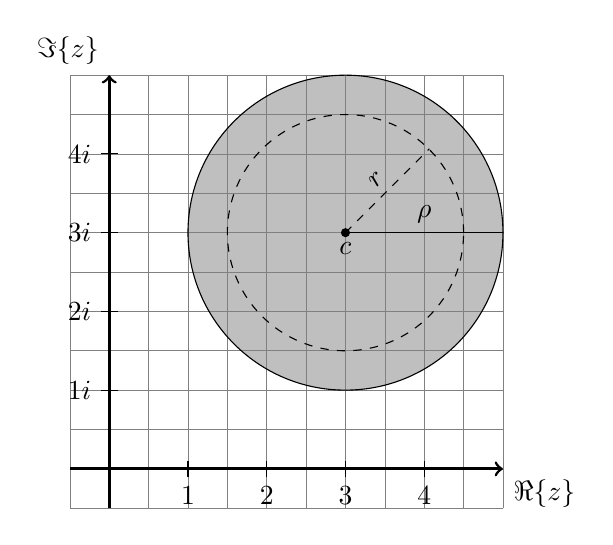
\begin{tikzpicture}
   % coords
   \coordinate (OR) at (0, 0);
   \coordinate (LX) at (-0.5, 0);
   \coordinate (RX) at (5, 0);
   \coordinate (TY) at (0, 5);
   \coordinate (BY) at (0, -0.5);

   % debugging grid
   \coordinate (BL) at (-0.5, -0.5);
   \coordinate (TR) at (5, 5);
   \draw[step=0.5cm, gray, very thin] (BL) grid (TR);

   % coordinate system
   \draw[->][line width=1.00pt] (LX) -- (RX) node[anchor=north west] {\(\Re\{z\}\)};
   \draw[->][line width=1.00pt] (BY) -- (TY) node[anchor=south east] {\(\Im\{z\}\)};
   \foreach \n in {1,2,...,4}{%
      \draw (\n,-3pt) node [below] {$\n$} -- (\n,3pt);
      \draw (-3pt,\n) node [left] {$\n i$} -- (3pt,\n);
   }

   \coordinate (c) at (3,3);
   \path[fill=gray, semitransparent] (c) circle (2);
   \draw[fill] (c) node[anchor=north]{\(c\)} circle [radius=0.05];
   \draw (c) circle (2);
   \draw (c) -- (5,3) node [midway, above, sloped, black] (TextNode) {\(\rho\)};

   \draw[dashed] (c) circle (1.5);
   \draw[dashed] (c) -- (4.065, 4.065) node [midway, above, sloped, black] (TextNode) {\(r\)};
\end{tikzpicture}

% \end{center}

\begin{theorem}[Power Series Convergence]\label{thm:conv_radius}
   Let \(\rho\) be the radius of convergence for \(\sum a_n z^n\).
   \[\forall |z| < \rho \implies \sum a_n z^n~\text{converges absolutely}\]
   \[\forall |z| > \rho \implies \sum a_n z^n~\text{diverges.}\]
\end{theorem}
\begin{remark}
   If \(\rho = 0\), diverges \(\sum a_nz^n~\forall z \neq 0\).

   If \(\rho = \infty\) converges \(\sum a_nz^n~\forall z \in \mathbb{C}\) and the convergence is uniform on \(\{z \in \mathbb{C} \mid |z| < r\}\).
\end{remark}
\begin{example}
   For \(\sum_{n=0}^\infty z^n\) is \(\rho = 1\).
   The series converges to 0 for all \(|z| < 1\) and diverges for all \(|z| \geq 1\).
\end{example}
\begin{example}
   For \(\sum_{n=0}^\infty \frac{1}{n} z^n\) is \(\rho = 1\).
   It converges for \(|z| < 1\), diverges for \(z = 1\) (like the harmonic series).
   For \(z = -1\) is it the alternating harmonic series and converges.
\end{example}

\begin{proposition}\label{pro:conv_rad_ratio_test}
   Let \(\rho\) be the radius of convergence of \(\sum a_n z^n\).
   \[\rho = \lim_{n \to \infty} \frac{|a_n|}{|a_{n+1}|}\]
\end{proposition}
\begin{remark}
   This proposition states that \(\rho\) can be calculated with the ratio test (\ref{pro:ratio_test}).
\end{remark}

\begin{theorem}
   Let \(\alpha \in \mathbb{C}\), \(\sum a_n (z - c)^n\) and \(\sum b_n (z-c)^n\) be power series with radius of convergence \(\rho_a\) respectively \(\rho_b\).
   \begin{enumerate}[label=\roman*, align=Center]
      \item \(\forall |z-c| < \rho_a: \alpha \sum a_n (z - c)^n = \sum \alpha a_n (z - c)^n\)
      \item \(\forall |z-c| < \min\{\rho_a, \rho_b\}: \sum a_n (z-c)^n + \sum b_n (z-c)^n = \sum (a_n + b_n)(z-c)^n\)
      \item \(\forall |z-c| < \min\{\rho_a, \rho_b\}:\)
            \[\sum a_n (z-c)^n \cdot \sum b_n (z-c)^n = \sum_{n=0}^\infty\left(\sum_{k=0}^\infty a_k \cdot b_{n-k}\right)(z-c)^n\]
   \end{enumerate}
\end{theorem}

\newpage

\subsection{Elementary Functions}
An \emph{elementary function} is a function of a single variable composed of particular simple functions.
They are typically defined as a sum, product, and/or composition of finitely many polynomials, rational functions, trigonometric and exponential functions, and their inverse functions.

\subsubsection{Exponential Function}
\begin{definition}[Exponential Function]
   Given \(z \in \mathbb{Z}\) we define \(\exp: \mathbb{C} \to \mathbb{C}\) by
   \[\exp(z) := \sum_{n = 0}^\infty \frac{z^n}{n!}\]
\end{definition}

\begin{proposition}[Properties]
   Let \(x, y, z \in \mathbb{C}\)
   \begin{enumerate}[label=\roman*, align=Center]
      \item The series has radius of convergence \(\rho = \infty\)
      \item \(\exp\) is continuous
      \item \(\exp(x + y) = \exp(x) \cdot \exp(y)\)
      \item \(\exp(-z) = \frac{1}{\exp(z)}\)
   \end{enumerate}
\end{proposition}

\begin{definition}[Eulers Number]
   \[e := \exp(1) = \sum_{n=0}^\infty \frac{1}{n!}\]
\end{definition}
\begin{remark}[Notation]
   From above we have \(e^z := \exp(z)\).
\end{remark}

Let \(z \in \mathbb{C}\), we see that
\[\exp(z) = \exp(x + iy) = \exp(x) \cdot \exp(iy)\]
 which means that the complex \(\exp\) function is characterized by
\[\exp: \mathbb{R} \to \mathbb{R} \qquad\text{and}\qquad \exp: i\mathbb{R} \to \mathbb{R}\]

\subsubsection{Logarithm}
\begin{proposition}
   Let \(\exp: \mathbb{R} \to \mathbb{R}\), then
   \begin{enumerate}[label=\roman*, align=Center]
      \item \(\exp\) is strictly increasing
      \item \(\im(\exp) = (0; \infty)\)
      \item \(\forall n \in \mathbb{N}: \lim_{x \to \infty} \frac{\exp(x)}{x^n} = \infty\)
      \item \(\lim_{x \to -\infty} \exp(x) = 0\)
   \end{enumerate}
\end{proposition}
\begin{remark}[Intuition]
   We would split (ii) into the following observations:
   \[\forall x < 0: \exp(x) \in (0; 1) \qquad \forall x > 0: \exp(x) \in (1; \infty) \qquad \exp(0) = 1\]
   Point (v) means that \(\exp\) grows faster than any other power.
\end{remark}

\begin{definition}[Logarithm]
   The inverse of \(\exp: \mathbb{R} \to (0; \infty)\) is
   \[\ln(x): (0; \infty) \to \mathbb{R} \qquad\text{where}\qquad \ln(x) = y \iff \exp(y) = x\]
\end{definition}

\begin{proposition}[Properties]
   Let \(x, y \in (0; \infty)\)
   \begin{enumerate}[label=\roman*, align=Center]
      \item \(\ln\) is continuous
      \item \(\ln\) is strictly increasing
      \item \(\lim_{x \to \infty} \ln(x) = \infty\)
      \item \(\lim_{x \to 0} \ln(x) = -\infty\)
      \item \(\ln(x \cdot y) = \ln(x) + \ln(y)\)
      \item \(\ln\left(\frac{x}{y}\right) = \ln(x) - \ln(y)\)
   \end{enumerate}
\end{proposition}
\begin{remark}
   From above we also have that \(\ln(1) = 0\).
\end{remark}

\subsubsection{Real Exponents}
Now that we have that \(x = \exp\big(\ln(x)\big)\) we can define \(x^r\) with \(r \in \mathbb{R}\).
First we need to check if everything remains the same as with whole exponents, so let \(n \in \mathbb{N}\) and \(x > 0\), then
\[x^n = \Big(\exp\big(\ln(x)\big)\Big)^n = \left(e^{\ln(x)}\right)^n = \exp\big(n \cdot \ln(x)\big)\]
\[x^{-n} = \frac{1}{x^n} = \frac{1}{\exp\big(n \cdot \ln(x)\big)} = \frac{1}{e^{n \cdot \ln(x)}} = e^{-n \cdot \ln(x)} = \exp\big(-n \cdot \ln(x)\big)\]
\[\sqrt[n]{x} = x^{\frac{1}{n}} = \Big(\exp\big(\ln(x)\big)\Big)^\frac{1}{n} = \exp\left(\frac{1}{n} \ln(x)\right)\]
and for \(p \in \mathbb{Z}\), \(q \in \mathbb{N}_{>0}\)
\[x^\frac{p}{q} = \Big(\exp\big(\ln(x)\big)\Big)^\frac{p}{q} = \exp\left(\frac{p}{q} \ln(x)\right)\]

\begin{definition}[Real Exponents]
   Given \(x > 0\) and \(r \in \mathbb{R}\)
   \[x^r := \exp\big(r \cdot \ln(x)\big)\]
\end{definition}

\begin{proposition}[Calculation Rules]
   Let \(x, y \in \mathbb{R}_{>0}\) and \(r, s \in \mathbb{R}\), then
   \begin{enumerate}[label=\roman*, align=Center]
      \item \(x^r \cdot x^s = x^{r + s}\)
      \item \(\frac{x^r}{x^s} = x^{r-s}\)
      \item \(x^r \cdot y^r = (x \cdot y)^r\)
      \item \((x^r)^s = x^{r \cdot s}\)
      \item \(\ln(x^r) = r \cdot \ln(x)\)
   \end{enumerate}
\end{proposition}

\begin{proposition}
   Let \(r \in \mathbb{R}_{>0}\) then
   \[\lim_{x \to \infty} x^{-r} \cdot \ln(x) = 0 \qquad\text{and}\qquad \lim_{x \to 0} x^r \cdot \ln(x) = 0\]
\end{proposition}
\begin{remark}
   This proposition states that \(\ln\) is damped by \(\frac{1}{x^n}\).
\end{remark}

\subsubsection{Trigonometric Functions}
\begin{definition}[Cosine]
   Given \(z \in \mathbb{C}\) we define \(\cos: \mathbb{C} \to \mathbb{C}\) by
   \[\cos(z) := \sum_{n=0}^\infty (-1)^n \frac{z^{2n}}{(2n)!}\]
\end{definition}

\begin{definition}[Sine]
   Given \(z \in \mathbb{C}\) we define \(\sin: \mathbb{C} \to \mathbb{C}\) by
   \[\sin(z) := \sum_{n=0}^\infty (-1)^n \frac{z^{2n + 1}}{(2n+1)!}\]
\end{definition}

\begin{proposition}[Properties]
   Let \(x, y \in \mathbb{R}\) and \(z \in \mathbb{C}\), then
   \begin{enumerate}[label=\roman*, align=Center]
      \item Both series have radius of convergence \(\rho = \infty\)
      \item \(\cos\) and \(\sin\) are continuous
      \item \(\cos(-z) = \cos(z)\)
      \item \(\sin(-z) = -\sin(z)\)
      \item \(\cos(x \pm y) = \cos(x) \cdot \cos(y) \mp \sin(x) \cdot \sin(y)\)
      \item \(\sin(x \pm y) = \sin(x) \cdot \cos(y) \pm \cos(x) \cdot \sin(y)\)
      \item \(\sin(x) - \sin(y) = 2 \cos\left(\frac{x+y}{2}\right) \cdot \sin\left(\frac{x-y}{2}\right)\)
      \item \(\cos(x) - \cos(y) = -2 \sin\left(\frac{x+y}{2}\right) \cdot \sin\left(\frac{x-y}{2}\right)\)
      \item \(\cos^2(z) + \sin^2(z) = 1\)
   \end{enumerate}
\end{proposition}

\subsubsection{Connecting Exponential and Trigonometric}
In this section we regard the imaginary part of the exponential function, for simplicity sake we define
\[\ixp: \mathbb{R} \to \mathbb{C} \qquad\text{by}\qquad \ixp(x) := \exp(ix)\]

\begin{proposition}
   Let \(\exp: i\mathbb{R} \to \mathbb{R}\) and \(x \in \mathbb{R}\), then
   \begin{enumerate}[label=\roman*, align=Center]
      \item \(\cos(x) = \Re\big(\exp(ix)\big)\)
      \item \(\sin(x) = \Im\big(\exp(ix)\big)\)
      \item \(\exp(ix) = \cos(x) + i \cdot \sin(x)\)
   \end{enumerate}
\end{proposition}

\begin{proposition}
   Let \(z \in \mathbb{C}\), then
   \[\cos(z) = \frac{\exp(iz) + \exp(-iz)}{2} \qquad\text{and}\qquad \sin(z) = \frac{\exp(iz) - \exp(-iz)}{2i}\]
\end{proposition}

\begin{theorem}[Unit Circle]
   \(\im(\ixp) = S^1 := \{z \in \mathbb{C} \mid \lvert z\rvert = 1\}\)
\end{theorem}

\begin{center}
   \begin{tikzpicture}[line cap=round,line join=round,>=triangle 45,x=1cm,y=1cm]
   \begin{axis}[
   x=5cm,y=5cm,
   axis lines=middle,
   ymajorgrids=true,
   xmajorgrids=true,
   xmin=-1.1, xmax=1.1,
   ymin=-1.1, ymax=1.1,
   xtick={-1,-0.8,...,1},
   ytick={-1,-0.8,...,1},]

   \draw [line width=2pt,color=black] (0,0) circle (5cm);

   \draw [line width=2pt, color=black] (0,0)-- (0.6,0.8);

   \draw [line width=1pt, dashed]  (0.6,0)-- (0.6,0.8);
   \draw [line width=1pt, dashed] (0,0.8)-- (0.6,0.8);

   \draw [line width=2pt,color=red] (0,0)-- (0.6,0);
   \draw [line width=2pt,color=blue] (0,0)-- (0,0.8);

   \draw [fill=grey] (0.6,0.8) circle (2.5pt);
   \draw (0.67, 0.87 ) node {\(e^{it}\)};
   \draw (-0.6, 1) node {\(\{z \in \mathbb{C} \mid |z| = 1\}\)};

   \draw (0.3, 0.05) node {\(\cos(t)\)};
   \draw (0.12, 0.4) node {\(\sin(t)\)};
   \end{axis}
\end{tikzpicture}

\end{center}

\begin{theorem}
   The set
   \[M := \{x \in (0; \infty) \mid \ixp(x) = 1\}\]
   has a positive minimum
   \[\pi := \frac{1}{2} \min(M)\]
\end{theorem}

\begin{definition}[Periodic Function]
   \(f: \mathbb{K} \to \mathbb{K}\) is \(p\)-periodic iff
   \[\forall x \in \mathbb{K}: f(x + p) = f(x)\]
\end{definition}

\begin{theorem}
   Let \(z \in \mathbb{C}\) and \(k \in \mathbb{Z}\), then
   \[\exp(z) = 1 \iff z = 2 \pi i \cdot k\]
   \[\exp(z) = -1 \iff z = (2k + 1)\pi i\]
\end{theorem}
\begin{remark}
   It follows that for \(k \in \mathbb{Z}\) holds \(\exp(z) = \exp(z + 2k\pi i)\) i.e. \(\exp\) is \(2\pi i\)-periodic.
\end{remark}

\begin{theorem}
   For \(x \in \mathbb{R}\) is \(\ixp: [x; x + 2\pi) \to S^1\) bijective.
\end{theorem}

\begin{proposition}[Properties]
   Let \(k \in \mathbb{Z}\) and \(z \in \mathbb{C}\), then
   \begin{enumerate}[label=\roman*, align=Center]
      \item \(\cos(z) = \cos(z + 2k\pi)\)
      \item \(\sin(z) = \sin(z + 2k\pi)\)
      \item \(\cos(z) = 0 \iff z = \frac{\pi}{2} + k\pi\)
      \item \(\sin(z) = 0 \iff z = k\pi\)
      \item \(\forall x \in (0; \pi): \sin(x) > 0\)
      \item \(\forall x \in \left(0; \frac{\pi}{2}\right): \cos(x) > 0\)
      \item \(\sin\) is strictly increasing on \(\left[0; \frac{\pi}{2}\right]\)
      \item \(\sin(z + \pi) = -\sin(z)\)
      \item \(\cos(z + \pi) = -\cos(z)\)
      \item \(\sin\left(\frac{\pi}{2} - z\right) = \cos(z)\)
      \item \(\cos\left(\frac{\pi}{2} - z\right) = \sin(z)\)
      \item \(\im(\cos) = \im(\sin) = [-1;1]\)
   \end{enumerate}
\end{proposition}

\begin{theorem}
   For \(x \in \mathbb{R}\) is \(\exp: \mathbb{R} + i[x; x + 2\pi) \to \mathbb{C}\setminus\{0\}\) bijective.
\end{theorem}
\begin{remark}
   From this are polar coordinates of complex numbers derived.
\end{remark}

\begin{theorem}
   For \(z \in \mathbb{C}\setminus\{0\}\)
   \[\exists! \alpha \in [0; 2\pi): z = \lvert z\rvert \exp(i \alpha)\]
\end{theorem}
\begin{remark}
   We call \(\alpha\) the \emph{argument} of \(z\): \(\alpha := \argu(z)\).
\end{remark}

\begin{theorem}
   For \(x \in \mathbb{C}\) has \(z^n = x\) \(n\) distinct solutions
   \[z_k = \lvert x\rvert^\frac{1}{n} \exp\left(\frac{i(\argu(x) + 2\pi k)}{n}\right)\]
\end{theorem}


\newpage

\section{Function Limits}
So far we only looked at limits of sequences, now we want to regard how \(f: X \to Y\) behave as \(x \to x_0\).

\begin{definition}[Function Limit]\label{def:func_limit}
   Given \(f: D \to \mathbb{R}\) and a limit point \(x_0 \in D\) of \(X\).
   \[\lim_{x \to x_0} f(x) = L :\iff \forall \varepsilon > 0~\exists \delta > 0: (\forall x \in D: \lvert x - x_0 \rvert < \delta \implies \lvert f(x) - L\rvert < \varepsilon\]
\end{definition}
\begin{remark}[Intuition]
   Note that we can rewrite
   \[\lvert x - x_0\rvert < \delta \iff -\delta < x - x_0 < \delta \iff x_0 - \delta < x < x_0 + \delta \iff x \in (x_0 - \delta; x_0 + \delta)\]
   Hence we can rewrite the condition above as
   \[\forall x \in (x_0 - \delta; x_0 + \delta): f(x) \in \big(L - \varepsilon; L + \varepsilon\big)\]
\end{remark}

\begin{center}
   \begin{tikzpicture}[line cap=round,line join=round,>=triangle 45,x=1cm,y=1cm]
   \begin{axis}[
   ticks=none,
   x=2cm, y=2cm,
   axis lines=middle,
   ymajorgrids=true,
   xmajorgrids=true,
   xmin=-0.4, xmax=6.1,
   ymin=-0.4, ymax=3.1]
      \fill[line width=2pt,color=gray,fill=gray,fill opacity=0.1] (0,2.2) -- (8,2.2) -- (8,1) -- (0,1) -- cycle;
      \draw[line width=2pt,color=blue,smooth,samples=100,domain=-0.3:7] plot(\x,{ln((\x)+1)});

      \draw [line width=1pt,dashed] (0,1.6079667094364514) -- (4.000000075430033,1.6094379275201067);
      \draw [line width=1pt,dashed] (4.000000075430033,1.6094379275201067)-- (4,0);
      \draw [line width=1pt] (3,0) -- (2.9996517855796725,1.3862073037254237);
      \draw [line width=1pt] (5,0) -- (5.000842962216623,1.7918999530625097);
      \draw [line width=1pt] (0,2.2) -- (8,2.2);
      \draw [line width=1pt] (8,1) -- (0,1);

      \draw [line width=4pt,color=orange] (2.9996517855796725,1.3862073037254237)-- (3.199034292788041,1.4348545685627394)-- (3.399609048748734,1.4815156844194872)-- (3.5985123484097543,1.5257328486695583)-- (3.799087104370447,1.5684257132365922)-- (4.000000075430033,1.6094379275201067)-- (4.200236616291833,1.6487041276851904)-- (4.402482828552198,1.6868586309676052)-- (4.6013861282132185,1.7230140900075834)-- (4.8002894278742385,1.7579078176649696)-- (5.000842962216623,1.7918999530625097);

      \draw [fill=blue] (0,2.2) circle (2.5pt);
      \draw (0.39, 2.33) node {\(L + \varepsilon\)};
      \draw [fill=blue] (0,1.6079667094364514) circle (2.5pt);
      \draw (0.29, 1.7408231122516713) node {\(L\)};
      \draw [fill=blue] (0,1) circle (2.5pt);
      \draw (0.39, 1.13) node {\(L - \varepsilon\)};

      \draw [fill=blue] (4.000000075430033,1.6094379275201067) circle (2.5pt);

      \draw [fill=blue] (5,0) circle (2.5pt);
      \draw (5, -0.15) node {\(x_0 + \delta\)};
      \draw [fill=blue] (4,0) circle (2.5pt);
      \draw (4, -0.15) node {\(x_0\)};
      \draw [fill=blue] (3,0) circle (2.5pt);
      \draw (3, -0.15) node {\(x_0 - \delta\)};
   \end{axis}
\end{tikzpicture}

\end{center}

\subsection{Calculation-Rules \& -Tricks}
\begin{proposition}[Calculation Rules]
   Let \(f: I \to \mathbb{R}\), \(g: I \to \mathbb{R}\) and \(c \in \mathbb{R}\)
   \begin{enumerate}[label=\roman*, align=Center]
      \item \(\lim_{x \to a}\big(f(x) \pm g(x)\big) = \lim_{x \to a}\big(f(x)\big) \pm \lim_{x \to a}\big(g(x)\big)\)
      \item \(\lim_{x \to a} c \cdot f(x) = c \cdot \lim_{x \to a} f(x)\)
      \item \(\lim_{x \to a} f(x) \cdot g(x) = \lim_{x \to a} f(x) \cdot \lim_{x \to a} g(x)\)
      \item \(\lim_{x \to a} \frac{f(x)}{g(x)} = \frac{\lim_{x \to a} f(x)}{\lim_{x \to a} g(x)}\)
   \end{enumerate}
\end{proposition}

\subsubsection{Root-Trick}
The following is a usefull method to determine limits which contain the root function.
We want to find \(\lim_{x \to \infty} \sqrt{x^2 + x} - x\).
\begin{equation*}
   \begin{split}
      \lim_{x \to \infty} \left(\sqrt{x^2 + x} - x\right) & = \lim_{x \to \infty} \left(\left(\sqrt{x^2 + x} - x\right) \frac{\left(\sqrt{x^2 + x} + x\right)}{\left(\sqrt{x^2 + x} + x\right)}\right) = \lim_{x \to \infty} \left(\frac{x^2 + x - x^2}{\sqrt{x^2 + x} + x}\right) =\\
                                                          & = \lim_{x \to \infty} \left(\frac{x}{\sqrt{x^2 + x} + x}\right) = \lim_{x \to \infty} \frac{x}{x \left(\frac{\sqrt{x^2 + x}}{x} + 1\right)} = \frac{1}{\lim_{x \to \infty}\left(\frac{\sqrt{x^2 + x}}{x} + 1\right)} =\\
                                                          & = \frac{1}{\lim_{x \to \infty}\left(\sqrt{\frac{x^2 + x}{x^2}}\right) + 1} = \frac{1}{\sqrt{\lim_{x \to \infty}\frac{x^2 \left(1 + \frac{1}{x}\right)}{x^2}} + 1} = \frac{1}{\sqrt{\lim_{x \to \infty}\left(1 + \frac{1}{x}\right)} + 1} =\\
                                                          & = \frac{1}{\sqrt{1} + 1} = \frac{1}{2}
   \end{split}
\end{equation*}

\subsubsection{Fundamental Limit \(e\)}
We know that
\[\lim_{x \to \infty} \left(1 + \frac{1}{x}\right)^x = e \qquad\text{and}\qquad \lim_{x \to 0} (1 + x)^{\frac{1}{x}} = e\]
From this follows (not trivially) a neat trick:
\[\lim_{x \to x_0} \left(1 + \frac{1}{\ast}\right)^* = e\]
where \(\ast\) is some term in \(x\) with \(\ast \xrightarrow{x \to x_0} \infty\).
Equivalently we have
\[\lim_{x \to x_0} (1 + \ast)^{\frac{1}{\ast}} = e\]
where \(\ast \xrightarrow{x \to x_0} 0\).
\begin{example}
   We want to find \(\lim_{x \to \infty} \left(1 - \frac{3}{x}\right)^{2x}\).
   \[\lim_{x \to \infty} \left(1 - \frac{3}{x}\right)^{2x} = \lim_{x \to \infty} \left(\left(1 + \frac{1}{-\frac{x}{3}}\right)^{-\frac{x}{3}}\right)^{-\frac{3}{x} \cdot 2x} = \lim_{x \to \infty} e^{-\frac{6x}{x}} = e^{-6}\]
\end{example}

\subsubsection{Fundamental Limit \(\sin(x)\)}
We know that
\[\lim_{x \to 0} \frac{\sin(x)}{x} = 1\]
From this follows a neat trick:
\[\lim_{x \to x_0} \frac{\sin(\ast)}{\ast} = 1\]
where \(\ast\) is some term in \(x\) with \(\ast \xrightarrow{x \to x_0} 0\).
\begin{example}
   We want to find \(\lim_{x \to 1} \frac{\sin(1-x^2)}{1-x}\)
   \[\lim_{x \to 1} \frac{\sin(1-x^2)}{1-x} = \lim_{x \to 1}\frac{\sin(1-x^2)}{1-x^2} \cdot \frac{1-x^2}{1-x} = 1 \cdot \lim_{x \to 1} \frac{(1-x)(1+x)}{1-x} = \lim_{x \to 1} 1 + x = 2\]
\end{example}

% TODO: l'hopital needed
\subsubsection{\(e^{\log}\) - Trick}
The following is a usefull method to determine limits \(\lim_{x \to x_0} f(x)^{g(x)}\).
The main idea is to rewrite
\[f(x)^{g(x)} = \exp\Big(\log\big(f(x)^{g(x)}\big)\Big) = \exp\Big(g(x) \cdot \log\big(f(x)\big)\Big)\]
as \(\exp\) is continuous, we can pull the limit into the argument.
\begin{example}
   We want to find \(\lim_{x \to 0} x^{\sin(x)}\)
\end{example}

\subsection{One-Sided Limits}
\begin{definition}[One-Sided Limit]\label{def:one-sided_limit}
   Given a limit point \(x_0 \in \mathbb{R}\) of \(D\) and \(f: D \to \mathbb{R}\).
   \[\lim_{x \uparrow x_0}f(x) = \lim_{x \to x_0} f|_{D \cap (-\infty; x_0)}\]
   \[\lim_{x \downarrow x_0}f(x) = \lim_{x \to x_0} f|_{D \cap (x_0; \infty)}\]
\end{definition}
\begin{remark}[Terminology]
   We call \(\lim_{x \uparrow x_0} f(x)\) a \emph{left-handed} and \(\lim_{x \downarrow x_0} f(x)\) a \emph{right-handed} limit.
\end{remark}
\begin{remark}
   From \cref{def:func_limit} we can equivalently write
   \[\lim_{x \uparrow x_0} f(x) = L \iff \forall \varepsilon~\exists \delta > 0: (x \in D: x_0- \delta < x < x_0 \implies |f(x) - L| < \varepsilon)\]
   \[\lim_{x \downarrow x_0} f(x) = L \iff \forall \varepsilon~\exists \delta > 0: (x \in D: x_0 < x < x_0 + \delta \implies |f(x) - L| < \varepsilon)\]
\end{remark}
\begin{example}
   We regard
   \[f(x) = \begin{cases}0 & x \leq 0\\ 1 & x > 0\end{cases}\]
   where we see that
   \[\lim_{x \uparrow 0} f(x) = 0 \qquad \lim_{x \downarrow 0} f(x) = 1\]
\end{example}
\begin{center}
   \begin{tikzpicture}[line cap=round,line join=round,>=triangle 45,x=1cm,y=1cm]
   \begin{axis}[
   x=4cm,y=4cm,
   axis lines=middle,
   ymajorgrids=true,
   xmajorgrids=true,
   xmin=-0.7,
   xmax=0.7,
   ymin=-0.1,
   ymax=1.1,
   xtick={-1,0,1},
   ytick={-1,0,1},]
   \draw[line width=2pt,color=blue] (-1.2292426079511276,0) -- (-1.2292426079511276,0);
   \draw[line width=2pt,color=blue] (-1.2292426079511276,0) -- (-1.2226596040846602,0);
   \draw[line width=2pt,color=blue] (-1.2226596040846602,0) -- (-1.2160766002181929,0);
   \draw[line width=2pt,color=blue] (-1.2160766002181929,0) -- (-1.2094935963517255,0);
   \draw[line width=2pt,color=blue] (-1.2094935963517255,0) -- (-1.2029105924852581,0);
   \draw[line width=2pt,color=blue] (-1.2029105924852581,0) -- (-1.1963275886187907,0);
   \draw[line width=2pt,color=blue] (-1.1963275886187907,0) -- (-1.1897445847523234,0);
   \draw[line width=2pt,color=blue] (-1.1897445847523234,0) -- (-1.183161580885856,0);
   \draw[line width=2pt,color=blue] (-1.183161580885856,0) -- (-1.1765785770193886,0);
   \draw[line width=2pt,color=blue] (-1.1765785770193886,0) -- (-1.1699955731529212,0);
   \draw[line width=2pt,color=blue] (-1.1699955731529212,0) -- (-1.1634125692864539,0);
   \draw[line width=2pt,color=blue] (-1.1634125692864539,0) -- (-1.1568295654199865,0);
   \draw[line width=2pt,color=blue] (-1.1568295654199865,0) -- (-1.1502465615535191,0);
   \draw[line width=2pt,color=blue] (-1.1502465615535191,0) -- (-1.1436635576870517,0);
   \draw[line width=2pt,color=blue] (-1.1436635576870517,0) -- (-1.1370805538205844,0);
   \draw[line width=2pt,color=blue] (-1.1370805538205844,0) -- (-1.130497549954117,0);
   \draw[line width=2pt,color=blue] (-1.130497549954117,0) -- (-1.1239145460876496,0);
   \draw[line width=2pt,color=blue] (-1.1239145460876496,0) -- (-1.1173315422211823,0);
   \draw[line width=2pt,color=blue] (-1.1173315422211823,0) -- (-1.1107485383547149,0);
   \draw[line width=2pt,color=blue] (-1.1107485383547149,0) -- (-1.1041655344882475,0);
   \draw[line width=2pt,color=blue] (-1.1041655344882475,0) -- (-1.0975825306217801,0);
   \draw[line width=2pt,color=blue] (-1.0975825306217801,0) -- (-1.0909995267553128,0);
   \draw[line width=2pt,color=blue] (-1.0909995267553128,0) -- (-1.0844165228888454,0);
   \draw[line width=2pt,color=blue] (-1.0844165228888454,0) -- (-1.077833519022378,0);
   \draw[line width=2pt,color=blue] (-1.077833519022378,0) -- (-1.0712505151559106,0);
   \draw[line width=2pt,color=blue] (-1.0712505151559106,0) -- (-1.0646675112894433,0);
   \draw[line width=2pt,color=blue] (-1.0646675112894433,0) -- (-1.0580845074229759,0);
   \draw[line width=2pt,color=blue] (-1.0580845074229759,0) -- (-1.0515015035565085,0);
   \draw[line width=2pt,color=blue] (-1.0515015035565085,0) -- (-1.0449184996900411,0);
   \draw[line width=2pt,color=blue] (-1.0449184996900411,0) -- (-1.0383354958235738,0);
   \draw[line width=2pt,color=blue] (-1.0383354958235738,0) -- (-1.0317524919571064,0);
   \draw[line width=2pt,color=blue] (-1.0317524919571064,0) -- (-1.025169488090639,0);
   \draw[line width=2pt,color=blue] (-1.025169488090639,0) -- (-1.0185864842241716,0);
   \draw[line width=2pt,color=blue] (-1.0185864842241716,0) -- (-1.0120034803577043,0);
   \draw[line width=2pt,color=blue] (-1.0120034803577043,0) -- (-1.005420476491237,0);
   \draw[line width=2pt,color=blue] (-1.005420476491237,0) -- (-0.9988374726247695,0);
   \draw[line width=2pt,color=blue] (-0.9988374726247695,0) -- (-0.9922544687583021,0);
   \draw[line width=2pt,color=blue] (-0.9922544687583021,0) -- (-0.9856714648918348,0);
   \draw[line width=2pt,color=blue] (-0.9856714648918348,0) -- (-0.9790884610253674,0);
   \draw[line width=2pt,color=blue] (-0.9790884610253674,0) -- (-0.9725054571589,0);
   \draw[line width=2pt,color=blue] (-0.9725054571589,0) -- (-0.9659224532924326,0);
   \draw[line width=2pt,color=blue] (-0.9659224532924326,0) -- (-0.9593394494259653,0);
   \draw[line width=2pt,color=blue] (-0.9593394494259653,0) -- (-0.9527564455594979,0);
   \draw[line width=2pt,color=blue] (-0.9527564455594979,0) -- (-0.9461734416930305,0);
   \draw[line width=2pt,color=blue] (-0.9461734416930305,0) -- (-0.9395904378265632,0);
   \draw[line width=2pt,color=blue] (-0.9395904378265632,0) -- (-0.9330074339600958,0);
   \draw[line width=2pt,color=blue] (-0.9330074339600958,0) -- (-0.9264244300936284,0);
   \draw[line width=2pt,color=blue] (-0.9264244300936284,0) -- (-0.919841426227161,0);
   \draw[line width=2pt,color=blue] (-0.919841426227161,0) -- (-0.9132584223606937,0);
   \draw[line width=2pt,color=blue] (-0.9132584223606937,0) -- (-0.9066754184942263,0);
   \draw[line width=2pt,color=blue] (-0.9066754184942263,0) -- (-0.9000924146277589,0);
   \draw[line width=2pt,color=blue] (-0.9000924146277589,0) -- (-0.8935094107612915,0);
   \draw[line width=2pt,color=blue] (-0.8935094107612915,0) -- (-0.8869264068948242,0);
   \draw[line width=2pt,color=blue] (-0.8869264068948242,0) -- (-0.8803434030283568,0);
   \draw[line width=2pt,color=blue] (-0.8803434030283568,0) -- (-0.8737603991618894,0);
   \draw[line width=2pt,color=blue] (-0.8737603991618894,0) -- (-0.867177395295422,0);
   \draw[line width=2pt,color=blue] (-0.867177395295422,0) -- (-0.8605943914289547,0);
   \draw[line width=2pt,color=blue] (-0.8605943914289547,0) -- (-0.8540113875624873,0);
   \draw[line width=2pt,color=blue] (-0.8540113875624873,0) -- (-0.8474283836960199,0);
   \draw[line width=2pt,color=blue] (-0.8474283836960199,0) -- (-0.8408453798295525,0);
   \draw[line width=2pt,color=blue] (-0.8408453798295525,0) -- (-0.8342623759630852,0);
   \draw[line width=2pt,color=blue] (-0.8342623759630852,0) -- (-0.8276793720966178,0);
   \draw[line width=2pt,color=blue] (-0.8276793720966178,0) -- (-0.8210963682301504,0);
   \draw[line width=2pt,color=blue] (-0.8210963682301504,0) -- (-0.814513364363683,0);
   \draw[line width=2pt,color=blue] (-0.814513364363683,0) -- (-0.8079303604972157,0);
   \draw[line width=2pt,color=blue] (-0.8079303604972157,0) -- (-0.8013473566307483,0);
   \draw[line width=2pt,color=blue] (-0.8013473566307483,0) -- (-0.7947643527642809,0);
   \draw[line width=2pt,color=blue] (-0.7947643527642809,0) -- (-0.7881813488978135,0);
   \draw[line width=2pt,color=blue] (-0.7881813488978135,0) -- (-0.7815983450313462,0);
   \draw[line width=2pt,color=blue] (-0.7815983450313462,0) -- (-0.7750153411648788,0);
   \draw[line width=2pt,color=blue] (-0.7750153411648788,0) -- (-0.7684323372984114,0);
   \draw[line width=2pt,color=blue] (-0.7684323372984114,0) -- (-0.761849333431944,0);
   \draw[line width=2pt,color=blue] (-0.761849333431944,0) -- (-0.7552663295654767,0);
   \draw[line width=2pt,color=blue] (-0.7552663295654767,0) -- (-0.7486833256990093,0);
   \draw[line width=2pt,color=blue] (-0.7486833256990093,0) -- (-0.7421003218325419,0);
   \draw[line width=2pt,color=blue] (-0.7421003218325419,0) -- (-0.7355173179660746,0);
   \draw[line width=2pt,color=blue] (-0.7355173179660746,0) -- (-0.7289343140996072,0);
   \draw[line width=2pt,color=blue] (-0.7289343140996072,0) -- (-0.7223513102331398,0);
   \draw[line width=2pt,color=blue] (-0.7223513102331398,0) -- (-0.7157683063666724,0);
   \draw[line width=2pt,color=blue] (-0.7157683063666724,0) -- (-0.7091853025002051,0);
   \draw[line width=2pt,color=blue] (-0.7091853025002051,0) -- (-0.7026022986337377,0);
   \draw[line width=2pt,color=blue] (-0.7026022986337377,0) -- (-0.6960192947672703,0);
   \draw[line width=2pt,color=blue] (-0.6960192947672703,0) -- (-0.6894362909008029,0);
   \draw[line width=2pt,color=blue] (-0.6894362909008029,0) -- (-0.6828532870343356,0);
   \draw[line width=2pt,color=blue] (-0.6828532870343356,0) -- (-0.6762702831678682,0);
   \draw[line width=2pt,color=blue] (-0.6762702831678682,0) -- (-0.6696872793014008,0);
   \draw[line width=2pt,color=blue] (-0.6696872793014008,0) -- (-0.6631042754349334,0);
   \draw[line width=2pt,color=blue] (-0.6631042754349334,0) -- (-0.6565212715684661,0);
   \draw[line width=2pt,color=blue] (-0.6565212715684661,0) -- (-0.6499382677019987,0);
   \draw[line width=2pt,color=blue] (-0.6499382677019987,0) -- (-0.6433552638355313,0);
   \draw[line width=2pt,color=blue] (-0.6433552638355313,0) -- (-0.636772259969064,0);
   \draw[line width=2pt,color=blue] (-0.636772259969064,0) -- (-0.6301892561025966,0);
   \draw[line width=2pt,color=blue] (-0.6301892561025966,0) -- (-0.6236062522361292,0);
   \draw[line width=2pt,color=blue] (-0.6236062522361292,0) -- (-0.6170232483696618,0);
   \draw[line width=2pt,color=blue] (-0.6170232483696618,0) -- (-0.6104402445031945,0);
   \draw[line width=2pt,color=blue] (-0.6104402445031945,0) -- (-0.6038572406367271,0);
   \draw[line width=2pt,color=blue] (-0.6038572406367271,0) -- (-0.5972742367702597,0);
   \draw[line width=2pt,color=blue] (-0.5972742367702597,0) -- (-0.5906912329037923,0);
   \draw[line width=2pt,color=blue] (-0.5906912329037923,0) -- (-0.584108229037325,0);
   \draw[line width=2pt,color=blue] (-0.584108229037325,0) -- (-0.5775252251708576,0);
   \draw[line width=2pt,color=blue] (-0.5775252251708576,0) -- (-0.5709422213043902,0);
   \draw[line width=2pt,color=blue] (-0.5709422213043902,0) -- (-0.5643592174379228,0);
   \draw[line width=2pt,color=blue] (-0.5643592174379228,0) -- (-0.5577762135714555,0);
   \draw[line width=2pt,color=blue] (-0.5577762135714555,0) -- (-0.5511932097049881,0);
   \draw[line width=2pt,color=blue] (-0.5511932097049881,0) -- (-0.5446102058385207,0);
   \draw[line width=2pt,color=blue] (-0.5446102058385207,0) -- (-0.5380272019720533,0);
   \draw[line width=2pt,color=blue] (-0.5380272019720533,0) -- (-0.531444198105586,0);
   \draw[line width=2pt,color=blue] (-0.531444198105586,0) -- (-0.5248611942391186,0);
   \draw[line width=2pt,color=blue] (-0.5248611942391186,0) -- (-0.5182781903726512,0);
   \draw[line width=2pt,color=blue] (-0.5182781903726512,0) -- (-0.5116951865061838,0);
   \draw[line width=2pt,color=blue] (-0.5116951865061838,0) -- (-0.5051121826397165,0);
   \draw[line width=2pt,color=blue] (-0.5051121826397165,0) -- (-0.49852917877324915,0);
   \draw[line width=2pt,color=blue] (-0.49852917877324915,0) -- (-0.49194617490678183,0);
   \draw[line width=2pt,color=blue] (-0.49194617490678183,0) -- (-0.4853631710403145,0);
   \draw[line width=2pt,color=blue] (-0.4853631710403145,0) -- (-0.4787801671738472,0);
   \draw[line width=2pt,color=blue] (-0.4787801671738472,0) -- (-0.4721971633073799,0);
   \draw[line width=2pt,color=blue] (-0.4721971633073799,0) -- (-0.46561415944091256,0);
   \draw[line width=2pt,color=blue] (-0.46561415944091256,0) -- (-0.45903115557444524,0);
   \draw[line width=2pt,color=blue] (-0.45903115557444524,0) -- (-0.4524481517079779,0);
   \draw[line width=2pt,color=blue] (-0.4524481517079779,0) -- (-0.4458651478415106,0);
   \draw[line width=2pt,color=blue] (-0.4458651478415106,0) -- (-0.4392821439750433,0);
   \draw[line width=2pt,color=blue] (-0.4392821439750433,0) -- (-0.43269914010857596,0);
   \draw[line width=2pt,color=blue] (-0.43269914010857596,0) -- (-0.42611613624210865,0);
   \draw[line width=2pt,color=blue] (-0.42611613624210865,0) -- (-0.4195331323756413,0);
   \draw[line width=2pt,color=blue] (-0.4195331323756413,0) -- (-0.412950128509174,0);
   \draw[line width=2pt,color=blue] (-0.412950128509174,0) -- (-0.4063671246427067,0);
   \draw[line width=2pt,color=blue] (-0.4063671246427067,0) -- (-0.39978412077623937,0);
   \draw[line width=2pt,color=blue] (-0.39978412077623937,0) -- (-0.39320111690977205,0);
   \draw[line width=2pt,color=blue] (-0.39320111690977205,0) -- (-0.38661811304330473,0);
   \draw[line width=2pt,color=blue] (-0.38661811304330473,0) -- (-0.3800351091768374,0);
   \draw[line width=2pt,color=blue] (-0.3800351091768374,0) -- (-0.3734521053103701,0);
   \draw[line width=2pt,color=blue] (-0.3734521053103701,0) -- (-0.3668691014439028,0);
   \draw[line width=2pt,color=blue] (-0.3668691014439028,0) -- (-0.36028609757743546,0);
   \draw[line width=2pt,color=blue] (-0.36028609757743546,0) -- (-0.35370309371096814,0);
   \draw[line width=2pt,color=blue] (-0.35370309371096814,0) -- (-0.3471200898445008,0);
   \draw[line width=2pt,color=blue] (-0.3471200898445008,0) -- (-0.3405370859780335,0);
   \draw[line width=2pt,color=blue] (-0.3405370859780335,0) -- (-0.3339540821115662,0);
   \draw[line width=2pt,color=blue] (-0.3339540821115662,0) -- (-0.32737107824509887,0);
   \draw[line width=2pt,color=blue] (-0.32737107824509887,0) -- (-0.32078807437863155,0);
   \draw[line width=2pt,color=blue] (-0.32078807437863155,0) -- (-0.31420507051216423,0);
   \draw[line width=2pt,color=blue] (-0.31420507051216423,0) -- (-0.3076220666456969,0);
   \draw[line width=2pt,color=blue] (-0.3076220666456969,0) -- (-0.3010390627792296,0);
   \draw[line width=2pt,color=blue] (-0.3010390627792296,0) -- (-0.2944560589127623,0);
   \draw[line width=2pt,color=blue] (-0.2944560589127623,0) -- (-0.28787305504629496,0);
   \draw[line width=2pt,color=blue] (-0.28787305504629496,0) -- (-0.28129005117982764,0);
   \draw[line width=2pt,color=blue] (-0.28129005117982764,0) -- (-0.2747070473133603,0);
   \draw[line width=2pt,color=blue] (-0.2747070473133603,0) -- (-0.268124043446893,0);
   \draw[line width=2pt,color=blue] (-0.268124043446893,0) -- (-0.2615410395804257,0);
   \draw[line width=2pt,color=blue] (-0.2615410395804257,0) -- (-0.25495803571395836,0);
   \draw[line width=2pt,color=blue] (-0.25495803571395836,0) -- (-0.24837503184749102,0);
   \draw[line width=2pt,color=blue] (-0.24837503184749102,0) -- (-0.24179202798102367,0);
   \draw[line width=2pt,color=blue] (-0.24179202798102367,0) -- (-0.23520902411455633,0);
   \draw[line width=2pt,color=blue] (-0.23520902411455633,0) -- (-0.22862602024808898,0);
   \draw[line width=2pt,color=blue] (-0.22862602024808898,0) -- (-0.22204301638162163,0);
   \draw[line width=2pt,color=blue] (-0.22204301638162163,0) -- (-0.2154600125151543,0);
   \draw[line width=2pt,color=blue] (-0.2154600125151543,0) -- (-0.20887700864868694,0);
   \draw[line width=2pt,color=blue] (-0.20887700864868694,0) -- (-0.2022940047822196,0);
   \draw[line width=2pt,color=blue] (-0.2022940047822196,0) -- (-0.19571100091575225,0);
   \draw[line width=2pt,color=blue] (-0.19571100091575225,0) -- (-0.1891279970492849,0);
   \draw[line width=2pt,color=blue] (-0.1891279970492849,0) -- (-0.18254499318281756,0);
   \draw[line width=2pt,color=blue] (-0.18254499318281756,0) -- (-0.1759619893163502,0);
   \draw[line width=2pt,color=blue] (-0.1759619893163502,0) -- (-0.16937898544988286,0);
   \draw[line width=2pt,color=blue] (-0.16937898544988286,0) -- (-0.16279598158341552,0);
   \draw[line width=2pt,color=blue] (-0.16279598158341552,0) -- (-0.15621297771694817,0);
   \draw[line width=2pt,color=blue] (-0.15621297771694817,0) -- (-0.14962997385048082,0);
   \draw[line width=2pt,color=blue] (-0.14962997385048082,0) -- (-0.14304696998401348,0);
   \draw[line width=2pt,color=blue] (-0.14304696998401348,0) -- (-0.13646396611754613,0);
   \draw[line width=2pt,color=blue] (-0.13646396611754613,0) -- (-0.12988096225107879,0);
   \draw[line width=2pt,color=blue] (-0.12988096225107879,0) -- (-0.12329795838461145,0);
   \draw[line width=2pt,color=blue] (-0.12329795838461145,0) -- (-0.11671495451814412,0);
   \draw[line width=2pt,color=blue] (-0.11671495451814412,0) -- (-0.11013195065167679,0);
   \draw[line width=2pt,color=blue] (-0.11013195065167679,0) -- (-0.10354894678520946,0);
   \draw[line width=2pt,color=blue] (-0.10354894678520946,0) -- (-0.09696594291874212,0);
   \draw[line width=2pt,color=blue] (-0.09696594291874212,0) -- (-0.09038293905227479,0);
   \draw[line width=2pt,color=blue] (-0.09038293905227479,0) -- (-0.08379993518580746,0);
   \draw[line width=2pt,color=blue] (-0.08379993518580746,0) -- (-0.07721693131934013,0);
   \draw[line width=2pt,color=blue] (-0.07721693131934013,0) -- (-0.0706339274528728,0);
   \draw[line width=2pt,color=blue] (-0.0706339274528728,0) -- (-0.06405092358640546,0);
   \draw[line width=2pt,color=blue] (-0.06405092358640546,0) -- (-0.05746791971993812,0);
   \draw[line width=2pt,color=blue] (-0.05746791971993812,0) -- (-0.05088491585347078,0);
   \draw[line width=2pt,color=blue] (-0.05088491585347078,0) -- (-0.044301911987003444,0);
   \draw[line width=2pt,color=blue] (-0.044301911987003444,0) -- (-0.037718908120536104,0);
   \draw[line width=2pt,color=blue] (-0.037718908120536104,0) -- (-0.031135904254068765,0);
   \draw[line width=2pt,color=blue] (-0.031135904254068765,0) -- (-0.024552900387601426,0);
   \draw[line width=2pt,color=blue] (-0.024552900387601426,0) -- (-0.017969896521134086,0);
   \draw[line width=2pt,color=blue] (-0.017969896521134086,0) -- (-0.011386892654666747,0);
   \draw[line width=2pt,color=blue] (-0.011386892654666747,0) -- (-0.004803888788199409,0);
   \draw[line width=2pt,color=blue] (0.0017791150782679298,1) -- (0.008362118944735267,1);
   \draw[line width=2pt,color=blue] (0.008362118944735267,1) -- (0.014945122811202607,1);
   \draw[line width=2pt,color=blue] (0.014945122811202607,1) -- (0.021528126677669946,1);
   \draw[line width=2pt,color=blue] (0.021528126677669946,1) -- (0.028111130544137285,1);
   \draw[line width=2pt,color=blue] (0.028111130544137285,1) -- (0.03469413441060462,1);
   \draw[line width=2pt,color=blue] (0.03469413441060462,1) -- (0.04127713827707196,1);
   \draw[line width=2pt,color=blue] (0.04127713827707196,1) -- (0.0478601421435393,1);
   \draw[line width=2pt,color=blue] (0.0478601421435393,1) -- (0.05444314601000664,1);
   \draw[line width=2pt,color=blue] (0.05444314601000664,1) -- (0.06102614987647398,1);
   \draw[line width=2pt,color=blue] (0.06102614987647398,1) -- (0.06760915374294131,1);
   \draw[line width=2pt,color=blue] (0.06760915374294131,1) -- (0.07419215760940864,1);
   \draw[line width=2pt,color=blue] (0.07419215760940864,1) -- (0.08077516147587598,1);
   \draw[line width=2pt,color=blue] (0.08077516147587598,1) -- (0.08735816534234331,1);
   \draw[line width=2pt,color=blue] (0.08735816534234331,1) -- (0.09394116920881064,1);
   \draw[line width=2pt,color=blue] (0.09394116920881064,1) -- (0.10052417307527797,1);
   \draw[line width=2pt,color=blue] (0.10052417307527797,1) -- (0.1071071769417453,1);
   \draw[line width=2pt,color=blue] (0.1071071769417453,1) -- (0.11369018080821264,1);
   \draw[line width=2pt,color=blue] (0.11369018080821264,1) -- (0.12027318467467997,1);
   \draw[line width=2pt,color=blue] (0.12027318467467997,1) -- (0.1268561885411473,1);
   \draw[line width=2pt,color=blue] (0.1268561885411473,1) -- (0.13343919240761465,1);
   \draw[line width=2pt,color=blue] (0.13343919240761465,1) -- (0.140022196274082,1);
   \draw[line width=2pt,color=blue] (0.140022196274082,1) -- (0.14660520014054934,1);
   \draw[line width=2pt,color=blue] (0.14660520014054934,1) -- (0.1531882040070167,1);
   \draw[line width=2pt,color=blue] (0.1531882040070167,1) -- (0.15977120787348403,1);
   \draw[line width=2pt,color=blue] (0.15977120787348403,1) -- (0.16635421173995138,1);
   \draw[line width=2pt,color=blue] (0.16635421173995138,1) -- (0.17293721560641873,1);
   \draw[line width=2pt,color=blue] (0.17293721560641873,1) -- (0.17952021947288607,1);
   \draw[line width=2pt,color=blue] (0.17952021947288607,1) -- (0.18610322333935342,1);
   \draw[line width=2pt,color=blue] (0.18610322333935342,1) -- (0.19268622720582076,1);
   \draw[line width=2pt,color=blue] (0.19268622720582076,1) -- (0.1992692310722881,1);
   \draw[line width=2pt,color=blue] (0.1992692310722881,1) -- (0.20585223493875546,1);
   \draw[line width=2pt,color=blue] (0.20585223493875546,1) -- (0.2124352388052228,1);
   \draw[line width=2pt,color=blue] (0.2124352388052228,1) -- (0.21901824267169015,1);
   \draw[line width=2pt,color=blue] (0.21901824267169015,1) -- (0.2256012465381575,1);
   \draw[line width=2pt,color=blue] (0.2256012465381575,1) -- (0.23218425040462484,1);
   \draw[line width=2pt,color=blue] (0.23218425040462484,1) -- (0.2387672542710922,1);
   \draw[line width=2pt,color=blue] (0.2387672542710922,1) -- (0.24535025813755953,1);
   \draw[line width=2pt,color=blue] (0.24535025813755953,1) -- (0.2519332620040269,1);
   \draw[line width=2pt,color=blue] (0.2519332620040269,1) -- (0.2585162658704942,1);
   \draw[line width=2pt,color=blue] (0.2585162658704942,1) -- (0.2650992697369615,1);
   \draw[line width=2pt,color=blue] (0.2650992697369615,1) -- (0.27168227360342884,1);
   \draw[line width=2pt,color=blue] (0.27168227360342884,1) -- (0.27826527746989616,1);
   \draw[line width=2pt,color=blue] (0.27826527746989616,1) -- (0.2848482813363635,1);
   \draw[line width=2pt,color=blue] (0.2848482813363635,1) -- (0.2914312852028308,1);
   \draw[line width=2pt,color=blue] (0.2914312852028308,1) -- (0.2980142890692981,1);
   \draw[line width=2pt,color=blue] (0.2980142890692981,1) -- (0.30459729293576543,1);
   \draw[line width=2pt,color=blue] (0.30459729293576543,1) -- (0.31118029680223275,1);
   \draw[line width=2pt,color=blue] (0.31118029680223275,1) -- (0.31776330066870007,1);
   \draw[line width=2pt,color=blue] (0.31776330066870007,1) -- (0.3243463045351674,1);
   \draw[line width=2pt,color=blue] (0.3243463045351674,1) -- (0.3309293084016347,1);
   \draw[line width=2pt,color=blue] (0.3309293084016347,1) -- (0.337512312268102,1);
   \draw[line width=2pt,color=blue] (0.337512312268102,1) -- (0.34409531613456934,1);
   \draw[line width=2pt,color=blue] (0.34409531613456934,1) -- (0.35067832000103666,1);
   \draw[line width=2pt,color=blue] (0.35067832000103666,1) -- (0.357261323867504,1);
   \draw[line width=2pt,color=blue] (0.357261323867504,1) -- (0.3638443277339713,1);
   \draw[line width=2pt,color=blue] (0.3638443277339713,1) -- (0.3704273316004386,1);
   \draw[line width=2pt,color=blue] (0.3704273316004386,1) -- (0.37701033546690593,1);
   \draw[line width=2pt,color=blue] (0.37701033546690593,1) -- (0.38359333933337325,1);
   \draw[line width=2pt,color=blue] (0.38359333933337325,1) -- (0.39017634319984057,1);
   \draw[line width=2pt,color=blue] (0.39017634319984057,1) -- (0.3967593470663079,1);
   \draw[line width=2pt,color=blue] (0.3967593470663079,1) -- (0.4033423509327752,1);
   \draw[line width=2pt,color=blue] (0.4033423509327752,1) -- (0.4099253547992425,1);
   \draw[line width=2pt,color=blue] (0.4099253547992425,1) -- (0.41650835866570984,1);
   \draw[line width=2pt,color=blue] (0.41650835866570984,1) -- (0.42309136253217716,1);
   \draw[line width=2pt,color=blue] (0.42309136253217716,1) -- (0.4296743663986445,1);
   \draw[line width=2pt,color=blue] (0.4296743663986445,1) -- (0.4362573702651118,1);
   \draw[line width=2pt,color=blue] (0.4362573702651118,1) -- (0.4428403741315791,1);
   \draw[line width=2pt,color=blue] (0.4428403741315791,1) -- (0.44942337799804644,1);
   \draw[line width=2pt,color=blue] (0.44942337799804644,1) -- (0.45600638186451375,1);
   \draw[line width=2pt,color=blue] (0.45600638186451375,1) -- (0.4625893857309811,1);
   \draw[line width=2pt,color=blue] (0.4625893857309811,1) -- (0.4691723895974484,1);
   \draw[line width=2pt,color=blue] (0.4691723895974484,1) -- (0.4757553934639157,1);
   \draw[line width=2pt,color=blue] (0.4757553934639157,1) -- (0.48233839733038303,1);
   \draw[line width=2pt,color=blue] (0.48233839733038303,1) -- (0.48892140119685035,1);
   \draw[line width=2pt,color=blue] (0.48892140119685035,1) -- (0.49550440506331767,1);
   \draw[line width=2pt,color=blue] (0.49550440506331767,1) -- (0.502087408929785,1);
   \draw[line width=2pt,color=blue] (0.502087408929785,1) -- (0.5086704127962524,1);
   \draw[line width=2pt,color=blue] (0.5086704127962524,1) -- (0.5152534166627197,1);
   \draw[line width=2pt,color=blue] (0.5152534166627197,1) -- (0.5218364205291871,1);
   \draw[line width=2pt,color=blue] (0.5218364205291871,1) -- (0.5284194243956545,1);
   \draw[line width=2pt,color=blue] (0.5284194243956545,1) -- (0.5350024282621219,1);
   \draw[line width=2pt,color=blue] (0.5350024282621219,1) -- (0.5415854321285892,1);
   \draw[line width=2pt,color=blue] (0.5415854321285892,1) -- (0.5481684359950566,1);
   \draw[line width=2pt,color=blue] (0.5481684359950566,1) -- (0.554751439861524,1);
   \draw[line width=2pt,color=blue] (0.554751439861524,1) -- (0.5613344437279914,1);
   \draw[line width=2pt,color=blue] (0.5613344437279914,1) -- (0.5679174475944587,1);
   \draw[line width=2pt,color=blue] (0.5679174475944587,1) -- (0.5745004514609261,1);
   \draw[line width=2pt,color=blue] (0.5745004514609261,1) -- (0.5810834553273935,1);
   \draw[line width=2pt,color=blue] (0.5810834553273935,1) -- (0.5876664591938608,1);
   \draw[line width=2pt,color=blue] (0.5876664591938608,1) -- (0.5942494630603282,1);
   \draw[line width=2pt,color=blue] (0.5942494630603282,1) -- (0.6008324669267956,1);
   \draw[line width=2pt,color=blue] (0.6008324669267956,1) -- (0.607415470793263,1);
   \draw[line width=2pt,color=blue] (0.607415470793263,1) -- (0.6139984746597303,1);
   \draw[line width=2pt,color=blue] (0.6139984746597303,1) -- (0.6205814785261977,1);
   \draw[line width=2pt,color=blue] (0.6205814785261977,1) -- (0.6271644823926651,1);
   \draw[line width=2pt,color=blue] (0.6271644823926651,1) -- (0.6337474862591325,1);
   \draw[line width=2pt,color=blue] (0.6337474862591325,1) -- (0.6403304901255998,1);
   \draw[line width=2pt,color=blue] (0.6403304901255998,1) -- (0.6469134939920672,1);
   \draw[line width=2pt,color=blue] (0.6469134939920672,1) -- (0.6534964978585346,1);
   \draw[line width=2pt,color=blue] (0.6534964978585346,1) -- (0.660079501725002,1);
   \draw[line width=2pt,color=blue] (0.660079501725002,1) -- (0.6666625055914693,1);
   \draw[line width=2pt,color=blue] (0.6666625055914693,1) -- (0.6732455094579367,1);
   \draw[line width=2pt,color=blue] (0.6732455094579367,1) -- (0.6798285133244041,1);
   \draw[line width=2pt,color=blue] (0.6798285133244041,1) -- (0.6864115171908715,1);
   \draw[line width=2pt,color=blue] (0.6864115171908715,1) -- (0.6929945210573388,1);
   \draw[line width=2pt,color=blue] (0.6929945210573388,1) -- (0.6995775249238062,1);
   \draw[line width=2pt,color=blue] (0.6995775249238062,1) -- (0.7061605287902736,1);
   \draw[line width=2pt,color=blue] (0.7061605287902736,1) -- (0.712743532656741,1);
   \draw[line width=2pt,color=blue] (0.712743532656741,1) -- (0.7193265365232083,1);
   \draw[line width=2pt,color=blue] (0.7193265365232083,1) -- (0.7259095403896757,1);
   \draw[line width=2pt,color=blue] (0.7259095403896757,1) -- (0.7324925442561431,1);
   \draw[line width=2pt,color=blue] (0.7324925442561431,1) -- (0.7390755481226104,1);
   \draw[line width=2pt,color=blue] (0.7390755481226104,1) -- (0.7456585519890778,1);
   \draw[line width=2pt,color=blue] (0.7456585519890778,1) -- (0.7522415558555452,1);
   \draw[line width=2pt,color=blue] (0.7522415558555452,1) -- (0.7588245597220126,1);
   \draw[line width=2pt,color=blue] (0.7588245597220126,1) -- (0.7654075635884799,1);
   \draw[line width=2pt,color=blue] (0.7654075635884799,1) -- (0.7719905674549473,1);
   \draw[line width=2pt,color=blue] (0.7719905674549473,1) -- (0.7785735713214147,1);
   \draw[line width=2pt,color=blue] (0.7785735713214147,1) -- (0.7851565751878821,1);
   \draw[line width=2pt,color=blue] (0.7851565751878821,1) -- (0.7917395790543494,1);
   \draw[line width=2pt,color=blue] (0.7917395790543494,1) -- (0.7983225829208168,1);
   \draw[line width=2pt,color=blue] (0.7983225829208168,1) -- (0.8049055867872842,1);
   \draw[line width=2pt,color=blue] (0.8049055867872842,1) -- (0.8114885906537516,1);
   \draw[line width=2pt,color=blue] (0.8114885906537516,1) -- (0.8180715945202189,1);
   \draw[line width=2pt,color=blue] (0.8180715945202189,1) -- (0.8246545983866863,1);
   \draw[line width=2pt,color=blue] (0.8246545983866863,1) -- (0.8312376022531537,1);
   \draw[line width=2pt,color=blue] (0.8312376022531537,1) -- (0.8378206061196211,1);
   \draw[line width=2pt,color=blue] (0.8378206061196211,1) -- (0.8444036099860884,1);
   \draw[line width=2pt,color=blue] (0.8444036099860884,1) -- (0.8509866138525558,1);
   \draw[line width=2pt,color=blue] (0.8509866138525558,1) -- (0.8575696177190232,1);
   \draw[line width=2pt,color=blue] (0.8575696177190232,1) -- (0.8641526215854906,1);
   \draw[line width=2pt,color=blue] (0.8641526215854906,1) -- (0.8707356254519579,1);
   \draw[line width=2pt,color=blue] (0.8707356254519579,1) -- (0.8773186293184253,1);
   \draw[line width=2pt,color=blue] (0.8773186293184253,1) -- (0.8839016331848927,1);
   \draw[line width=2pt,color=blue] (0.8839016331848927,1) -- (0.89048463705136,1);
   \draw[line width=2pt,color=blue] (0.89048463705136,1) -- (0.8970676409178274,1);
   \draw[line width=2pt,color=blue] (0.8970676409178274,1) -- (0.9036506447842948,1);
   \draw[line width=2pt,color=blue] (0.9036506447842948,1) -- (0.9102336486507622,1);
   \draw[line width=2pt,color=blue] (0.9102336486507622,1) -- (0.9168166525172295,1);
   \draw[line width=2pt,color=blue] (0.9168166525172295,1) -- (0.9233996563836969,1);
   \draw[line width=2pt,color=blue] (0.9233996563836969,1) -- (0.9299826602501643,1);
   \draw[line width=2pt,color=blue] (0.9299826602501643,1) -- (0.9365656641166317,1);
   \draw[line width=2pt,color=blue] (0.9365656641166317,1) -- (0.943148667983099,1);
   \draw[line width=2pt,color=blue] (0.943148667983099,1) -- (0.9497316718495664,1);
   \draw[line width=2pt,color=blue] (0.9497316718495664,1) -- (0.9563146757160338,1);
   \draw[line width=2pt,color=blue] (0.9563146757160338,1) -- (0.9628976795825012,1);
   \draw[line width=2pt,color=blue] (0.9628976795825012,1) -- (0.9694806834489685,1);
   \draw[line width=2pt,color=blue] (0.9694806834489685,1) -- (0.9760636873154359,1);
   \draw[line width=2pt,color=blue] (0.9760636873154359,1) -- (0.9826466911819033,1);
   \draw[line width=2pt,color=blue] (0.9826466911819033,1) -- (0.9892296950483707,1);
   \draw[line width=2pt,color=blue] (0.9892296950483707,1) -- (0.995812698914838,1);
   \draw[line width=2pt,color=blue] (0.995812698914838,1) -- (1.0023957027813053,1);
   \draw[line width=2pt,color=blue] (1.0023957027813053,1) -- (1.0089787066477727,1);
   \draw[line width=2pt,color=blue] (1.0089787066477727,1) -- (1.01556171051424,1);
   \draw[line width=2pt,color=blue] (1.01556171051424,1) -- (1.0221447143807074,1);
   \draw[line width=2pt,color=blue] (1.0221447143807074,1) -- (1.0287277182471748,1);
   \draw[line width=2pt,color=blue] (1.0287277182471748,1) -- (1.0353107221136422,1);
   \draw[line width=2pt,color=blue] (1.0353107221136422,1) -- (1.0418937259801095,1);
   \draw[line width=2pt,color=blue] (1.0418937259801095,1) -- (1.048476729846577,1);
   \draw[line width=2pt,color=blue] (1.048476729846577,1) -- (1.0550597337130443,1);
   \draw[line width=2pt,color=blue] (1.0550597337130443,1) -- (1.0616427375795117,1);
   \draw[line width=2pt,color=blue] (1.0616427375795117,1) -- (1.068225741445979,1);
   \draw[line width=2pt,color=blue] (1.068225741445979,1) -- (1.0748087453124464,1);
   \draw[line width=2pt,color=blue] (1.0748087453124464,1) -- (1.0813917491789138,1);
   \draw[line width=2pt,color=blue] (1.0813917491789138,1) -- (1.0879747530453812,1);
   \draw[line width=2pt,color=blue] (1.0879747530453812,1) -- (1.0945577569118485,1);
   \draw[line width=2pt,color=blue] (1.0945577569118485,1) -- (1.101140760778316,1);
   \draw[line width=2pt,color=blue] (1.101140760778316,1) -- (1.1077237646447833,1);
   \draw[line width=2pt,color=blue] (1.1077237646447833,1) -- (1.1143067685112507,1);
   \draw[line width=2pt,color=blue] (1.1143067685112507,1) -- (1.120889772377718,1);
   \draw[line width=2pt,color=blue] (1.120889772377718,1) -- (1.1274727762441854,1);
   \draw[line width=2pt,color=blue] (1.1274727762441854,1) -- (1.1340557801106528,1);
   \draw[line width=2pt,color=blue] (1.1340557801106528,1) -- (1.1406387839771202,1);
   \draw[line width=2pt,color=blue] (1.1406387839771202,1) -- (1.1472217878435875,1);
   \draw[line width=2pt,color=blue] (1.1472217878435875,1) -- (1.153804791710055,1);
   \draw[line width=2pt,color=blue] (1.153804791710055,1) -- (1.1603877955765223,1);
   \draw[line width=2pt,color=blue] (1.1603877955765223,1) -- (1.1669707994429896,1);
   \draw[line width=2pt,color=blue] (1.1669707994429896,1) -- (1.173553803309457,1);
   \draw[line width=2pt,color=blue] (1.173553803309457,1) -- (1.1801368071759244,1);
   \draw[line width=2pt,color=blue] (1.1801368071759244,1) -- (1.1867198110423918,1);
   \draw[line width=2pt,color=blue] (1.1867198110423918,1) -- (1.1933028149088591,1);
   \draw[line width=2pt,color=blue] (1.1933028149088591,1) -- (1.1998858187753265,1);
   \draw[line width=2pt,color=blue] (1.1998858187753265,1) -- (1.206468822641794,1);
   \draw[line width=2pt,color=blue] (1.206468822641794,1) -- (1.2130518265082613,1);
   \draw[line width=2pt,color=blue] (1.2130518265082613,1) -- (1.2196348303747286,1);
   \draw[line width=2pt,color=blue] (1.2196348303747286,1) -- (1.226217834241196,1);
   \draw[line width=2pt,color=blue] (1.226217834241196,1) -- (1.2328008381076634,1);
   \draw[line width=2pt,color=blue] (1.2328008381076634,1) -- (1.2393838419741308,1);
   \draw[line width=2pt,color=blue] (1.2393838419741308,1) -- (1.2459668458405981,1);
   \draw[line width=2pt,color=blue] (1.2459668458405981,1) -- (1.2525498497070655,1);
   \draw[line width=2pt,color=blue] (1.2525498497070655,1) -- (1.2591328535735329,1);
   \draw[line width=2pt,color=blue] (1.2591328535735329,1) -- (1.2657158574400003,1);
   \draw[line width=2pt,color=blue] (1.2657158574400003,1) -- (1.2722988613064676,1);
   \draw[line width=2pt,color=blue] (1.2722988613064676,1) -- (1.278881865172935,1);
   \draw[line width=2pt,color=blue] (1.278881865172935,1) -- (1.2854648690394024,1);
   \draw[line width=2pt,color=blue] (1.2854648690394024,1) -- (1.2920478729058698,1);
   \draw[line width=2pt,color=blue] (1.2920478729058698,1) -- (1.2986308767723371,1);
   \draw[line width=2pt,color=blue] (1.2986308767723371,1) -- (1.3052138806388045,1);
   \draw[line width=2pt,color=blue] (1.3052138806388045,1) -- (1.3117968845052719,1);
   \draw[line width=2pt,color=blue] (1.3117968845052719,1) -- (1.3183798883717393,1);
   \draw[line width=2pt,color=blue] (1.3183798883717393,1) -- (1.3249628922382066,1);
   \draw[line width=2pt,color=blue] (1.3249628922382066,1) -- (1.331545896104674,1);
   \draw[line width=2pt,color=blue] (1.331545896104674,1) -- (1.3381288999711414,1);
   \draw[line width=2pt,color=blue] (1.3381288999711414,1) -- (1.3447119038376087,1);
   \draw[line width=2pt,color=blue] (1.3447119038376087,1) -- (1.3512949077040761,1);
   \draw[line width=2pt,color=blue] (1.3512949077040761,1) -- (1.3578779115705435,1);
   \draw[line width=2pt,color=blue] (1.3578779115705435,1) -- (1.3644609154370109,1);
   \draw[line width=2pt,color=blue] (1.3644609154370109,1) -- (1.3710439193034782,1);
   \draw[line width=2pt,color=blue] (1.3710439193034782,1) -- (1.3776269231699456,1);
   \draw[line width=2pt,color=blue] (1.3776269231699456,1) -- (1.384209927036413,1);
   \draw[line width=2pt,color=blue] (1.384209927036413,1) -- (1.3907929309028804,1);
   \draw[line width=2pt,color=blue] (1.3907929309028804,1) -- (1.3973759347693477,1);

   \draw [fill=blue] (0,0) circle (2.5pt);
   \draw [color=black] (0,1) circle (2.5pt);
\end{axis}
\end{tikzpicture}

\end{center}

\newpage

\section{Continuity}
In this sections we regard functions
\[f: D \subset (X, \|\ldots\|) \to (Y, \|\ldots\|)\]

\begin{theorem}[Continuity Definitions are Equivalent]
   \[\text{\cref{def:neigh_cont}} \iff \text{\cref{def:eps_delt_cont}} \iff \text{\cref{def:seq_cont}}\]
\end{theorem}

\begin{definition}[Set of Continuous Functions]
   \(C^0(D, Y)\) the set of continuous functions in \(Y\).
\end{definition}

\subsection{In Terms of Function Limits}
\begin{definition}[\(\varepsilon-\delta\) Continuity]\label{def:eps_delt_cont}
   \(f: D \to \mathbb{R}\) is continuous in \(x_0 \in D\) iff
   \[\forall \varepsilon > 0~\exists \delta > 0: (\forall x \in D: |x-x_0| < \delta \implies |f(x) - f(x_0)| < \varepsilon)\]
\end{definition}
\begin{remark}[Intuition]
   A \emph{continuous function} is a function that does not have any abrupt changes in value, known as \emph{discontinuities}.
   More precisely, sufficiently small changes in the input of a continuous function result in arbitrarily small changes in its output.
\end{remark}
\begin{remark}[Terminology]
   \(f\) is \emph{continuous} (on \(D\)) iff \(f\) is continuous in all \(x_0 \in D\).

   \(f\) is \emph{discontinuous} in \(x_0\) iff
   \[\exists \varepsilon > 0~\forall \delta > 0: (\exists x \in D: |x - x_0| < \delta~\text{but}~|f(x) - f(x_0)| \geq \varepsilon)\]
\end{remark}

With \cref{def:func_limit} we see that
\begin{theorem}[Function Continuity]
   Let \(f: D \to \mathbb{R}\) and \(x_0 \in D\), then is
   \[f~\text{continuous in}~x_0 \iff \lim_{x \to x_0} f(x) = f(x_0)\]
\end{theorem}

This makes sense, because if \(f\) does not approach \(f(x_0\), there must be a ''gap in the function graph``.
This becomes apparant when regarding both one-sided limits, approaching the same point.

\begin{theorem}
   Let \(x_0 \in \mathbb{R}\) be a limit point of \(D\) and \(f: D \to \mathbb{R}\).
   \[\lim_{x \to x_0} f(x) = L \iff \lim_{x \uparrow x_0} f(x) = L = \lim_{x \downarrow x_0} f(x)\]
\end{theorem}

\begin{definition}[Jump Discontinuity]
   Given \(D \subset \mathbb{R}\) and \(f: D \to \mathbb{R}\)
   \[x_0 \in \mathbb{R}: x_0 \in \overline{D \cap (-\infty; x_0)} \cap \overline{D \cap (x_0; \infty)}\]
   is a \emph{jump discontinuity} iff
   \[\lim_{x \uparrow a} f(x) \neq \lim_{x \downarrow a} f(x)\]
\end{definition}

\begin{theorem}
   Let \(f:D \to \mathbb{R}\) be monotonic. \(f\) has countable jump discontinuities.
\end{theorem}

\begin{proposition}\label{pro:one_sided_lim_incr}
   Let \(f: [a; b] \to \mathbb{R}\) and \(c \in (a; b)\).

   If \(f\) is increasing, then
   \[\lim_{x \uparrow c} f(x) = \sup\{f(x) \mid x < c\} \qquad\text{and}\qquad \lim_{x \downarrow c} f(x) = \inf\{f(x) \mid x > c\}\]

   If \(f\) is decreasing, then
   \[\lim_{x \uparrow c} f(x) = \inf\{f(x) \mid x < c\} \qquad\text{and}\qquad \lim_{x \downarrow c} f(x) = \sup\{f(x) \mid x > c\}\]
\end{proposition}
\begin{example}
   \[f(c_1) = \lim_{x \uparrow c_1} f(x) = f(c_1^-) < f(c_1^+)\]
   \[f(c_2) = \lim_{x \to c_2} f(x) = f(c_2^-) = f(c_2^+)\]
   \[f(c_3^-) < f(c_3) < f(c_3^+)\]
\end{example}
\begin{center}
   \begin{tikzpicture}[line cap=round,line join=round,>=triangle 45,x=1cm,y=1cm]
   \begin{axis}[
   ticks=none,
   x=1.5cm,y=1.5cm,
   axis lines=middle,
   ymajorgrids=true,
   xmajorgrids=true,
   xmin=-0.9, xmax=7.5,
   ymin=-0.5, ymax=4.9]

      \draw [line width=0.5pt,dashed] (7,0)-- (6.999347663225158,4.808375546139909);
      \draw [line width=0.5pt,dashed] (1,0)-- (1,1);

      \draw [fill=blue] (1,0) circle (2.5pt);
      \draw (1, -0.2) node {\(a\)};
      \draw [fill=blue] (7,0) circle (2.5pt);
      \draw (7, -0.2) node {\(b\)};

      \draw [line width=4pt, color=green] (1,1)-- (3,2);
      \draw [line width=4pt, color=green] (3,2.1741614881443576)-- (4.792997852271268,2.683669545697946);
      \draw [line width=4pt, color=green] (5.2,3.4324016315214996)-- (6.999347663225158,4.808375546139909);

      \draw [line width=0.5pt, dashed] (0,2) -- (3,2);
      \draw [line width=0.5pt, dashed] (4,0)-- (3.9960481823364784,2.4572039769957392);
      \draw [line width=0.5pt, dashed] (3.9960481823364784,2.4572039769957392)-- (0,2.451192594490506);
      \draw [line width=0.5pt, dashed] (3,0)-- (3,2);
      \draw [line width=0.5pt, dashed] (5,0)-- (5.000511853340461,3.0404031012859707);
      \draw [line width=0.5pt, dashed] (5.000511853340461,3.0404031012859707)-- (0,3.041252304933857);
      \draw [line width=0.5pt, dashed] (4.792997852271268,2.683669545697946)-- (0,2.674060594245076);
      \draw [line width=0.5pt, dashed] (5.2,3.4324016315214996)-- (0,3.4344860163850863);

      \draw [fill=red] (3,0) circle (2.5pt);
      \draw (3, -0.2) node {$c_1$};
      \draw [fill=red] (0,2) circle (2.5pt);
      \draw (-0.4, 2) node {$f(c_1)$};
      \draw [fill=red] (3,2) circle (2.5pt);

      \draw [fill=orange] (4,0) circle (2.5pt);
      \draw (4, -0.2) node {$c_2$};
      \draw [fill=orange] (3.9960481823364784,2.4572039769957392) circle (2.5pt);
      \draw [fill=orange] (0,2.451192594490506) circle (2.5pt);
      \draw (-0.4, 2.4) node {$f(c_2)$};

      \draw [fill=yellow] (5,0) circle (2.5pt);
      \draw (5, -0.2) node {$c_3$};
      \draw [fill=yellow] (4.792997852271268,2.683669545697946) circle (2.5pt);
      \draw [fill=yellow] (5.000511853340461,3.0404031012859707) circle (2.5pt);
      \draw [fill=yellow] (5.2,3.4324016315214996) circle (2.5pt);

      \draw [fill=yellow] (0,2.674060594245076) circle (2.5pt);
      \draw (-0.4, 2.7) node {\(f(c_3^-)\)};
      \draw [fill=yellow] (0,3.041252304933857) circle (2.5pt);
      \draw (-0.4, 3.04) node {\(f(c_3)\)};
      \draw [fill=yellow] (0,3.4344860163850863) circle (2.5pt);
      \draw (-0.4, 3.43) node {\(f(c_3^+)\)};
   \end{axis}
\end{tikzpicture}

\end{center}

\subsection{In Terms of Sequences}
\begin{definition}[Sequence Continuity]\label{def:seq_cont}
   \(f: D \to \mathbb{R}\) is continuous in \(x_0 \in D\) iff
   \[\forall (x_n) \in (D\setminus\{x_0\})^\mathbb{N}: \lim_{n \to \infty} x_n = x_0 \implies \lim_{n \to \infty} f(x_n) = f(x_0)\]
\end{definition}
\begin{remark}
   This definition allows us interchange \(\lim f(x) = f(\lim(x))\).
\end{remark}

\begin{proposition}[Function Limit = Sequence Limit]
   Let \(x_0 \in X\) be a limit point of \(D\) and \(f: D \to \mathbb{R}\)
   \[\lim_{x \to x_0} f(x) = L \iff \forall (x_n) \in (D\setminus\{x_0\})^\mathbb{N}: \left(\lim_{n \to \infty} x_n = x_0 \implies  \lim_{n \to \infty} f(x_n) = L\right)\]
\end{proposition}

\subsection{In Terms of Topology}
\begin{definition}[Neighbourhood Continuity]\label{def:neigh_cont}
   \(f: D \to Y\) is continuous in \(x_0 \in D\) iff
   \[\forall V \in \mathcal{U}\big(f(x_0)\big)~\exists U \in \mathcal{U}(x_0): f(U \cap D) \subset V\]
\end{definition}
\begin{remark}
   Equivalently \(x \in U \implies f(x) \in V\)
\end{remark}

\begin{theorem}
   Given \(D' \subset D\), the following statements are equivalent
   \begin{enumerate}[label=\roman*, align=Center]
      \item \(f: D \to Y\) is continuous on \(D'\)
      \item Pre-images of open sets in \(Y\) are relatively open in \(D'\).
      \item Pre-images of closed sets in \(Y\) are relatively closed in \(D'\)
   \end{enumerate}
\end{theorem}

\begin{definition}[One-Sided Continuity]
   \(f: D \to \mathbb{R}\) is
   \[\text{left-continuous in}~x_0 \in D \iff \forall V \in \mathcal{U}\big(f(x_0)\big) \exists \delta > 0: f\big(D \cap (x_0 - \delta; x_0]\big) \subset V\]
   \[\text{right-continuous in}~x_0 \in D \iff \forall V \in \mathcal{U}\big(f(x_0)\big) \exists \delta > 0: f\big(D \cap [x_0; x_0 + \delta)\big) \subset V\]
\end{definition}

\begin{proposition}
   \(f: D \to \mathbb{R}\) is continuous in \(x_0 \in D\) iff it is left- and right-continuous in \(x_0\).
\end{proposition}

\subsection{Properties}
\begin{proposition}[Calculation Rules]
   Let \(f, g: D \to Y\) be continuous in \(x_0 \in D\), then is
   \begin{enumerate}[label=\roman*, align=Center]
      \item \(\alpha \cdot f: D \to Y \quad\text{where}\quad (\alpha \cdot f)(x) := \alpha \cdot f(x)\)
      \item \(f + g: D \to Y \quad\text{where}\quad (f + g)(x) := f(x) + g(x)\)
      \item \(f \cdot g: D \to \mathbb{K} \quad\text{where}\quad (f \cdot g)(x) := f(x) \cdot g(x)\)
      \item If \(g(x_0) \neq 0\)
         \[\frac{f}{g}: D \to \mathbb{K} \quad\text{where}\quad \left(\frac{f}{g}\right)(x) := \frac{f(x)}{g(x)}\]
   \end{enumerate}
   also continuous in \(x_0\).
\end{proposition}

\begin{corollary}
   Polynomials and rational functions are continuous.
\end{corollary}

\begin{proposition}[Composition is Continuous]\label{pro:contin_continuation}
   Let \(f: D_f \to Y\) and \(g: D_g \to Z\) such that \(\im(f) \subset D_g\).

   If \(f\) continuous at \(x_0 \in D_f\) and \(g\) at \(f(x_0) \in D_g\) then is
   \[g \circ f: D_f \to Z~\text{continuous in}~x_0\]
\end{proposition}
\begin{example}
   Let \(f(x) = x^2 + 3\) and \(g(x) = \sqrt{x}\).

   \(h(x) = (g \circ f)(x) = \sqrt{x^2 + 3}\) is continuous since \(f\) and \(g\) both are.
\end{example}

\begin{theorem}[Vector Functions]
   \(f := (f_1, f_2, \ldots, f_n): D \to \mathbb{K}^n\) is continuous in \(x_0 \in D\) iff
   \[\forall i \in [1; n]: f_i~\text{is continuous in}~x_0\]
\end{theorem}

\begin{theorem}[Complex Functions]
   \(f: D \to \mathbb{C}\) is continuous in \(x_0 \in D\) iff
   \[\Re(f)~\text{and}~\Im(f)~\text{are continuous in}~x_0\]
\end{theorem}

\begin{proposition}[Continuous Continuation]
   Let \(x_0\) be a limit point of \(D\) and assume there exists \(y := \lim_{x \to x_0} f(x)\).
   We define \(\tilde{f}: D \cup \{x_0\} \to Y\) by
   \[\tilde{f}(x) := \begin{cases}f(x) & \text{if}~x \in D\\ y & \text{if}~x = x_0\end{cases}\]
   then is \(\tilde{f}\) continuous in \(x_0\).
\end{proposition}

\subsection{Uniform Continuity}
Continuity itself is a local property of a function—that is, a function \(f\) is continuous, or not, at a particular point, and this can be determined by looking only at the values of the function in an (arbitrarily small) neighbourhood of that point.
When we speak of a function being continuous on an interval, we mean only that it is continuous at each point of the interval.
In contrast, uniform continuity is a global property of \(f\), in the sense that the standard definition refers to pairs of points rather than individual points.

\begin{definition}[Uniform Continuity]
   \(f: D \to Y\) is uniform continuous iff
   \[\forall \varepsilon > 0~\exists \delta > 0: (\forall x,y \in D': |x - y| < \delta \implies |f(x) - f(y)| < \varepsilon)\]
\end{definition}
\begin{remark}[Intuition]
   A function \(f\) is uniformly continuous if, it is possible to guarantee that \(f(x)\) and \(f(y)\) be as close to each other as we please by requiring only that \(x\) and \(y\) are sufficiently close to each other.
\end{remark}
\begin{remark}
   The difference to regular continuity is that for uniform continuity \(\delta\) does not depend on \(x_0\) but only on \(\varepsilon\).
   This means that the same \(\delta\) must be applicabale to all \(x \in D\).

   As this is a more strict requirement we have that every uniformly continuous function is also continuous.
\end{remark}

\section{Functions in R}
\begin{theorem}[Intermediate Value]\label{thm:intmd_value}
   Let \(f: [a; b] \to \mathbb{R}\) be continuous and \(f(a) < 0 < f(b)\).
   \[\exists \xi \in (a;b): f(\xi) = 0\]
\end{theorem}
\begin{remark}
   More in general: if \(f(a) < f(c) < f(b)\) then \(\exists \xi \in (a;b): f(\xi) = f(c)\).
\end{remark}

% TODO intervall types --> merge with foundations and equivalent reformulations (function limit)
\begin{theorem}
   Let \(f: [a;b] \to \mathbb{R}\) be continuous and strictly increasing, then is
   \begin{enumerate}[label=\roman*, align=Center]
      \item \(f\big([a;b]\big)\) an intervall of the same type as \([a;b]\).
      \item \(f:[a;b] \xrightarrow{\sim} f\big([a;b]\big)\)
      \item \(f^{-1}\) is continuous as strictly increasing.
   \end{enumerate}
\end{theorem}
\begin{remark}
   The same holds for decreasing \(f\).
\end{remark}
\begin{example}
   Let \(n \in \mathbb{N}: n \geq 2\) and \(f(x) := x^n\).
   First we show that \(f\) is strictly increasing, let \(x \in \mathbb{R}_{\geq 0}: x < y\), then
   \[f(y) - f(x) = y^n - x^n = y^n \left(1 - \left(\frac{x}{y}\right)^n\right)\]
   Recall that by the geometric series we have
   \[(1- q^n) = (1-q) \sum_{l=0}^{n-1} q^l = (1-q)\left(1 + \sum_{l=1}^{n-1} q^l\right)\]
   hence
   \[y^n \left(1 - \left(\frac{x}{y}\right)^n\right) = y^n \left(1 - \frac{x}{y}\right) \sum_{j=0}^{n-1} \left(\frac{x}{y}\right)^{n-1-j} > 0\]
   Therefor we have an inverse which is continuous and strictly increasing
   \[\sqrt[n]{x} := f^{-1}(x)\]
\end{example}

\newpage

\section{Differential Calculus}
Let \(D \subset \mathbb{K}\), \(x_0 \in D\) be an accumulation point of \(D\) and \((Y, \|\ldots\|)\).

\subsection{Definition \& Basic Properties}
When we differentiate a function \(f\) we want to calculate the slope of \(f\) at \(x_0\), which is the tangent to the function graph at \(x_0\).
To do this we start of by calculating the slope of the secant from \(\big(x_0, f(x_0)\big)\) to \(\big(x_0 + h, f(x_0) + h\big)\) through.
\[\frac{f(x_0 + h) - f(x_0)}{h}\]
Then we let \(h \to 0\) which makes the point \(\big(x_0 + h, f(x_0) + h\big)\) move along the function graph until it coincides with \(\big(x_0, f(x_0)\big)\).
At this point the secant coincides (never but close enough) the tangent, then the fraction above gives us the slope of the tangent.
\begin{center}
   \begin{tikzpicture}[line cap=round,line join=round,>=triangle 45,x=1cm,y=1cm]
   \begin{axis}[
   x=1.95cm,y=1.95cm,
   axis lines=middle,
   ymajorgrids=true,
   xmajorgrids=true,
   xmin=-0.9, xmax=6.9,
   ymin=-0.9, ymax=2.5,
   xtick={-1,0,...,9},
   ytick={-1,0,...,5},]

      \fill[line width=2pt,color=grey,fill=grey,fill opacity=0.3] (1.992250618110671,0.689264963553256) -- (6.004283509389274,1.792473132741205) -- (6.0042835093893,0.6892649635533) -- cycle;

      \draw[line width=3pt,color=black,smooth,samples=100,domain=0.3:7] plot(\x,{ln((\x))});

      \draw [line width=1.2pt,dashed] (6.004283509389274,1.792473132741205)-- (0,1.7979325541006292);
      \draw [line width=1.2pt,dashed] (1.992250618110671,0.689264963553256)-- (0,0.6865550452377207);
      \draw [line width=1.2pt,dashed] (1.9922506,0)-- (1.992250618110671,0.689264963553256);
      \draw [line width=1.2pt,dashed] (6.0042835093893,0)-- (6.004283509389274,1.792473132741205);

      \draw [line width=2pt,color=green,domain=-2.7782759088017714:9.763751218410293] plot(\x,{(--0.5674865476121775--1.103208169187949*\x)/4.0120328912786025});
      \draw [line width=2pt,color=blue,domain=-2.7782759088017714:9.763751218410293] plot(\x,{(-0.31073503644674405--0.5019448812862405*\x)/1});
      \draw (5.6, 2.3) node {\(f'(x_0)\)};

      \draw [->,line width=1pt] (5.76,-0.3156320939175) -- (2.1362418130313,-0.3156320939175);
      \draw [->,line width=1pt] (-0.4544428683875,1.6857552136163) -- (-0.4544428683875,0.7962497436013);

      \draw [fill=blue] (0, 1.7979325541006292) circle (2.5pt);
      \draw (-0.45, 1.8) node {\(f(x_0 + h)\)};
      \draw [fill=blue] (0,0.6865550452377207) circle (2.5pt);
      \draw (-0.4, 0.7) node {\(f(x_0)\)};

      \draw [fill=blue] (1.9922506,0) circle (2.5pt);
      \draw (2, -0.35) node {\(x_0\)};
      \draw [fill=blue] (6.0042835093893,0) circle (2.5pt);
      \draw (6.050065881097502,-0.3) node {\(x_0 + h\)};

      \draw [fill=red] (1.992250618110671, 0.689264963553256) circle (2.5pt);
      \draw [fill=red] (6.004283509389274,1.792473132741205) circle (2.5pt);
      \draw (4.204342030816293,-0.4101420501065896) node {\(h \to 0\)};
      \draw (-0.6, 1.346631253173085) node {\rotatebox{90}{\(h \to 0\)}};
   \end{axis}
\end{tikzpicture}

\end{center}

\begin{definition}[Differentiable Function]
   \(f: D \to Y\) is differentiable at \(x_0 \in D\) if
   \[\frac{df}{dx}(x_0) := \lim_{h \to 0} \frac{f(x_0 + h) - f(x_0)}{h}\]
   exists.
\end{definition}
\begin{remark}[Terminology]
   \(f\) is differentiable on \(D\) if \(f\) is differentiable in all \(x_0 \in D\).
   We call \(\frac{df}{dx}\) the \emph{derivative} of \(f\) at \(x_0\).
\end{remark}
\begin{remark}[Notation]
   For the derivative of \(f\) in \(x_0\) we write
   \[f'(x_0) \qquad\qquad Df(x_0) \qquad\qquad \lim_{x \to x_0} \frac{f(x) - f(x_0)}{x - x_0}\]
\end{remark}

\begin{proposition}[Derivative\(\implies\)Continuity]\label{pro:deri_impl_cont}
   If \(f: D \to \mathbb{R}\) is differentiable in \(x_0 \in D\) then is \(f\) also continuous in \(x_0\).
\end{proposition}

\begin{proposition}
   Let \(f: D \to Y\) be differentiable in \(x_0 \in D\), then
   \begin{enumerate}[label=\roman*, align=Center]
      \item
         \[\exists c \in Y: \lim_{x \to x_0} \frac{f(x) - f(x_0) - c \cdot (x - x_0)}{x - x_0} = 0\]
      \item There is \(c \in Y\) and \(r: D \to Y\) which is continuous in \(x_0\) and \(r(x_0) = 0\) such that
         \[\forall x \in D: f(x) = f(x_0) + c \cdot (x - x_0) + r(x) \cdot (x - x_0)\]
   \end{enumerate}
   Then is
   \[\frac{d}{dx}f(x_0) = c\]
\end{proposition}
